\documentclass[UTF8]{article}
% 中文支持
\usepackage[UTF8]{ctex}	
% pdf调用 封面
\usepackage{pdfpages}
% color宏包
\usepackage{color}  
% 导入图片
\usepackage{caption}
\usepackage{graphicx, subfig}
% 防止图片乱跑
\usepackage{float}
% 支持数学符号
\usepackage{amsmath}
% 支持代码块
\usepackage{listings}
% pdf加入大纲
\usepackage{hyperref}
% 大纲去红框
\hypersetup{hidelinks,
	colorlinks=true,
	allcolors=black,
	pdfstartview=Fit,
	breaklinks=true
}

% 绘制三线表
\usepackage{booktabs}    
% 消除警告
\usepackage{lmodern}

% 绘图
\usepackage{tikz}
\usetikzlibrary{positioning, shapes.geometric}

% 设置页面的环境,a4纸张大小,左右上下边距信息
\usepackage[a4paper, left=31.8mm, right=31.8mm, top=25.4mm, bottom=25.4mm]{geometry}

% 代码块的基本设置
\lstset{
 columns=fixed,       
 numbers=left,                                        % 在左侧显示行号
 numberstyle=\tiny\color{gray},                       % 设定行号格式
 frame=none,                                          % 不显示背景边框
 backgroundcolor=\color[RGB]{245,245,244},            % 设定背景颜色
 keywordstyle=\color[RGB]{40,40,255},                 % 设定关键字颜色
 numberstyle=\footnotesize\color{darkgray},           
 commentstyle=\it\color[RGB]{0,96,96},                % 设置代码注释的格式
 stringstyle=\rmfamily\slshape\color[RGB]{128,0,0},   % 设置字符串格式
 showstringspaces=false,                              % 不显示字符串中的空格
 language=matlab,                                        % 设置语言
}

% \begin{titlepage}
% % 封面信息
% 
\includepdf[pages={1}]{cover.pdf}
% \end{titlepage}

% 生成目录
% \tableofcontents
% \cleardoublepage

% 导入图片
% \begin{figure}[H]
%     \centering % 居中 
%     % 图片文件的相对路径
%     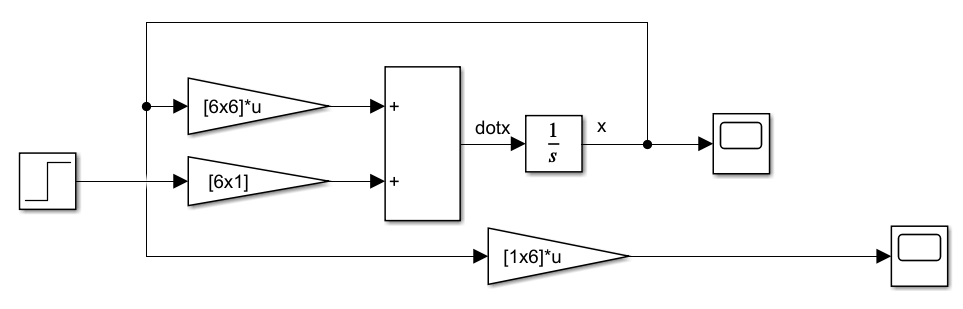
\includegraphics[width=.8\textwidth]{figure/exp1_1_model.png} 
%     \caption{Simulink模型} % caption是图片的标题
%     % \label{img} % 此处的label相当于一个图片的专属标志,目的是方便上下文的引用
% \end{figure}

% 导入代码
% \begin{lstlisting}
% a
% \end{lstlisting}

\begin{document}
\begin{titlepage}
% 封面信息
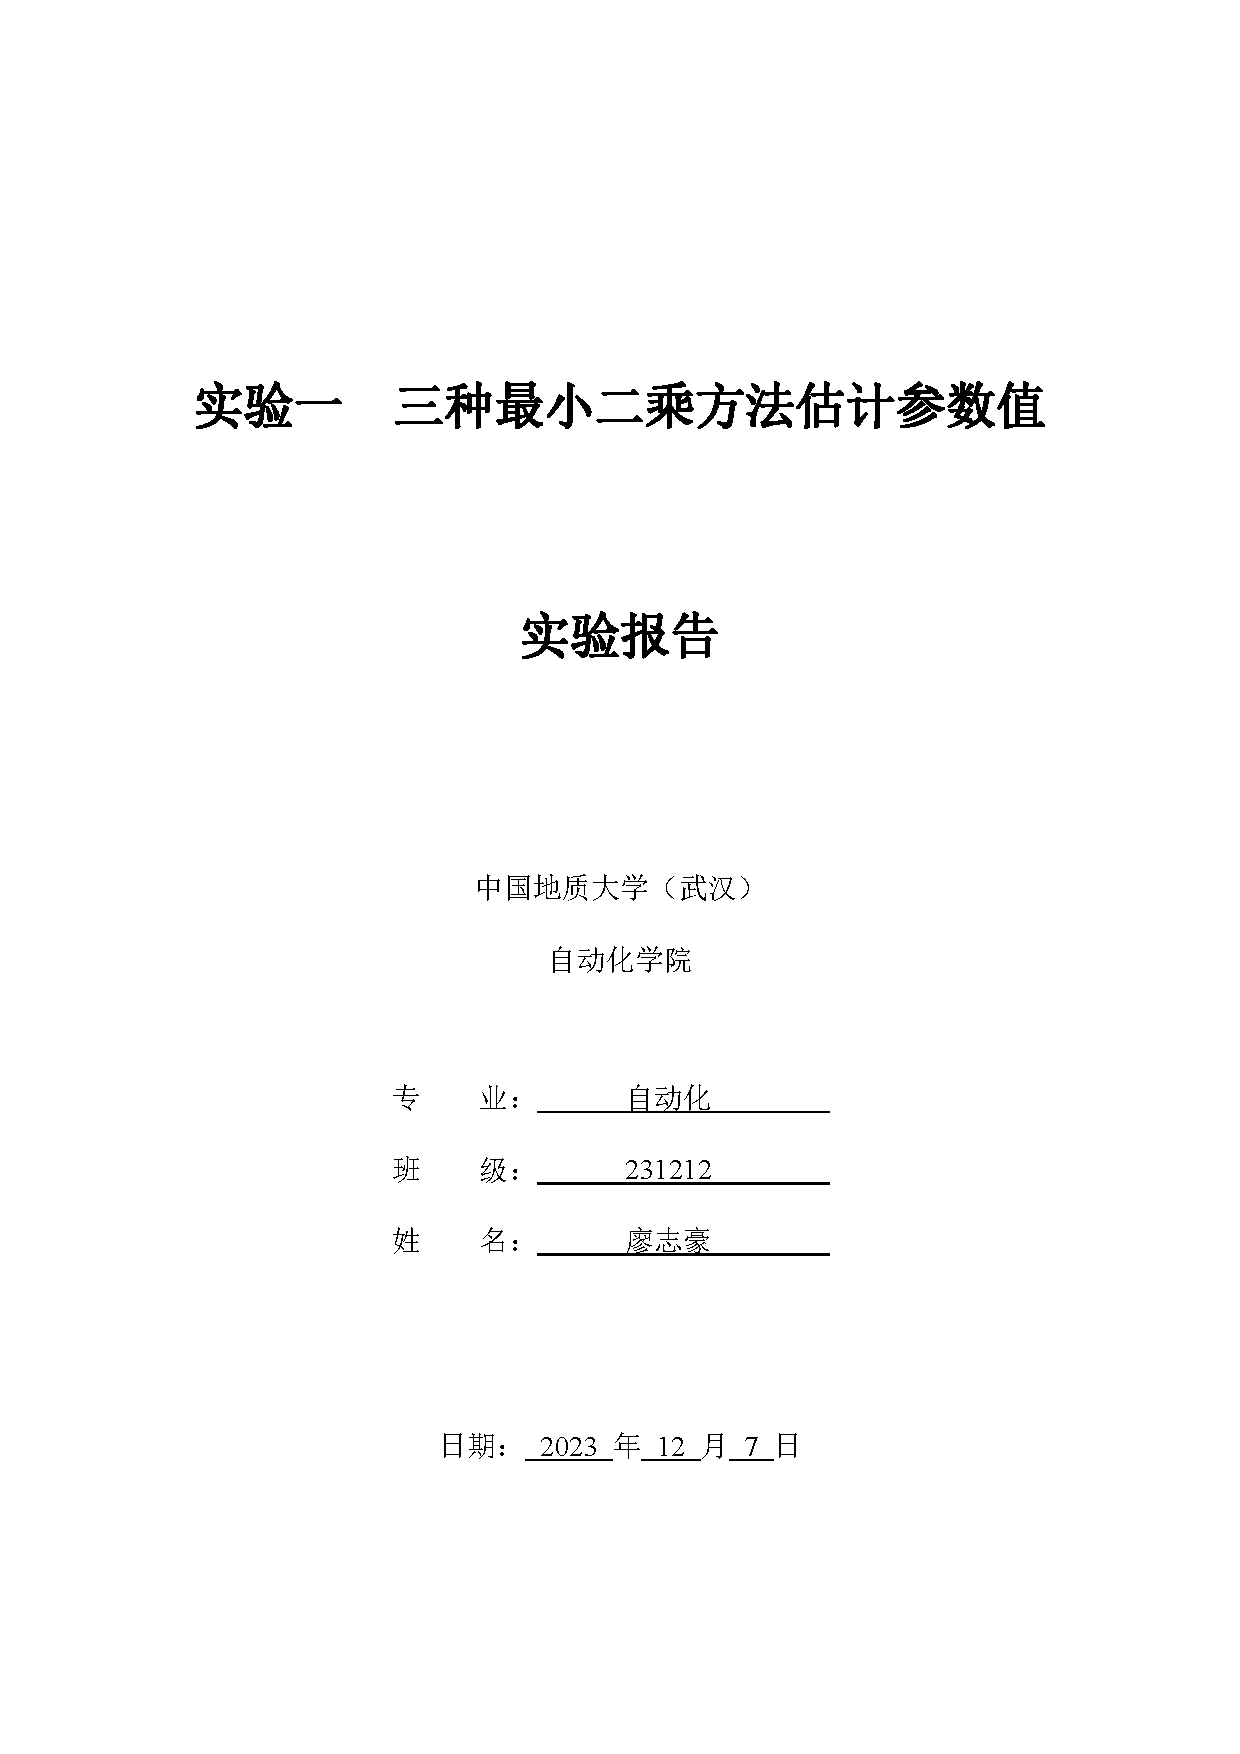
\includepdf[pages={1}]{cover/实验一封面.pdf}
\end{titlepage}

% 三种最小二乘方法估计参数值
%
\section{实验题目}
设单输入-单输出系统的差分方程为:
% 无编号单行公式
\begin{equation*}
    z(k) + a_1z(k-1) + a_2z(k-2) = b_1u(k-1) + b_2u(k-2) + V(k)
\end{equation*}
\begin{equation*}
    V(k) = c_1v(k) + c_2v(k-1) + c_3v(k-2)
\end{equation*}

取真值:$a_1 = 1.6,\ a_2 = 0.7,\ b_1 = 1.0,\ b_2 = 0.4,\ c_1 = 1.1,\ c_2 = 1.4,\ c_3 = 0.3$,输入信号采用4阶M序列,幅值为1。当$v(k)$的均值为0,方差分别为0.1和0.5的高斯噪声时,分别用一般最小二乘法、递推最小二乘法和增广递推最小二乘法估计参数$\theta$。并通过对三种方法的辨识结果的分析和比较,说明上述三种参数辨识方法的优缺点。

%
\section{实验目的}
\begin{enumerate}
    \item 掌握最小二乘法估计参数值的原理;
    \item 掌握三种最小二乘方法的实现和估计参数;
    \item 掌握三种最小二乘方法的优缺点,能够选择适合的方法估计参数值。
\end{enumerate}


%
\section{实验主要原理}
%%
\subsection{最小二乘法简介}
高斯的最小二乘基本原理:成对等精度地测得一组数据$t_i, y_i(i = 1,2,...,m)$,试找出一条最佳的拟合曲线,使得这条拟合曲线上的各点的值与测量值差的平方在所有拟合曲线中最小。即对于系统的观测输出$y(k)$:
\begin{equation*}
    y(k) = x(k) + v(k)
\end{equation*}

其中,$x(k)$表示系统的真实输出,$v(k)$表示系统输出的测量误差,则基于最小二乘法,应使得误差平方之和:
\begin{equation*}
    J = \sum_{k = 1}^m w(k) | y(k) - x(k) |^2
\end{equation*}
的值达到最小,其中$w(k)$代表权重值。

%%
\subsection{一般最小二乘法}
对于单输入-单输出系统:
\begin{equation*}
    y(k) = -\sum_{i = 1}^n a_iy(k - i) + \sum_{i = 0}^n b_iu(k - i) + \xi(k)
\end{equation*}
其中$\xi(k)$代表测量噪声。对该系统分别测出$n + N$个输入输出值:
\begin{equation*}
    y(1), y(2), ..., y(n + N)
\end{equation*}
\begin{equation*}
    u(1), u(2), ..., u(n + N)
\end{equation*}
则可以写出$N$个方程:
\begin{equation*}
    y(n+1) = -\sum_{i = 1}^n a_iy(n+1-i) + \sum_{i=0}^n b_iu(n+1-i) + \xi(n+1)
\end{equation*}
\begin{equation*}
    y(n+2) = -\sum_{i = 1}^n a_iy(n+2-i) + \sum_{i=0}^n b_iu(n+2-i) + \xi(n+2)
\end{equation*}
\begin{equation*}
    \vdots
\end{equation*}
\begin{equation*}
    y(n+N) = -\sum_{i = 1}^n a_iy(n+N-i) + \sum_{i=0}^n b_iu(n+N-i) + \xi(n+N)
\end{equation*}
定义以下变量:
\begin{equation*}
    y = 
    \begin{bmatrix}
        y(n+1) \\
        y(n+2) \\
        \vdots \\
        y(n+N) 
    \end{bmatrix}, \quad
    \theta = 
    \begin{bmatrix}
        a_1 \\
        \vdots \\
        a_n \\
        b_0 \\
        \vdots \\
        b_n
    \end{bmatrix}, \quad 
    \xi = 
    \begin{bmatrix}
        \xi(n+1) \\
        \xi(n+2) \\
        \vdots \\
        \xi(n+N)
    \end{bmatrix}
\end{equation*}
\begin{equation*}
    \Phi = 
    \begin{bmatrix}
        -y(n) & \dots & -y(1) & u(n+1) & \dots & u(1) \\
        -y(n+1) & \dots & -y(2) & u(n+2) & \dots & u(2) \\
        \vdots & & \vdots & \vdots & \vdots & \vdots \\
        -y(n+N-1) & \dots & -y(N) & u(n+N) & \dots & u(N)
    \end{bmatrix}
\end{equation*}
则可以得到:
\begin{equation*}
    y = \Phi\theta + \xi
\end{equation*}
定义残差变量:
\begin{equation*}
    e = y - \hat{y} = y - \Phi\hat{\theta}
\end{equation*}
最小二乘估计要求残差的平方和最小,即按照指标函数:
\begin{equation*}
    J = e^Te = (y - \Phi\hat{\theta})^T(y - \Phi\hat{\theta})
\end{equation*}
为最小来确定估值$\hat{\theta}$。求$J$对$\hat{\theta}$的偏导数并令其等于0可得$\theta$的最小二乘估计:
\begin{equation*}
    \hat{\theta} = (\Phi^T\Phi)^{-1}\Phi^Ty
\end{equation*}
$J$为极小值的充分条件是:
\begin{equation*}
    \frac{\partial^2 J}{\partial \hat{\theta}^2} = 2\Phi^T\Phi > 0
\end{equation*}
即矩阵$\Phi^T\Phi$为正定矩阵。

%%
\subsection{递推最小二乘法}
递推最小二乘法采用参数递推估计,其大致思路为:
\begin{center}
    当前估计值$\hat{\theta}(k)$ = 上次估计值$\hat{\theta}(k+1)$ + 修正项
\end{center}
递推最小二乘算法的计算公式如下:
\begin{equation*}
    \hat{\theta}_{m+1} = \hat{\theta}_{m} + K_{m+1}[z(m+1) - h(m+1)\hat{\theta}_m]
\end{equation*}
\begin{align*}
    P_{m+1} &= P_m - P_m h^T(m+1) [w^{-1}(m+1) + h(m+1) P_m h^T(m+1)]^{-1} h(m+1) P_m \\
    &= P_m - K_{m+1} K_{m+1}^T[w^{-1}(m+1) + h(m+1) P_m h^T(m+1)]
\end{align*}
\begin{equation*}
    K_{m+1} = P_m h^T(m+1) [w^{-1}(m+1) + h(m+1) P_m h^T(m+1)]^{-1}
\end{equation*}
其中:
\begin{itemize}
    \item $\hat{\theta}_m$:前一时刻的参数估值
    \item $z(m+1)$:当前时刻的量测值
    \item $h(m+1) \hat{\theta}_m$:在前一量测的基础上对在$(m+1)$的预测
    \item $z(m+1) - h(m+1) \hat{\theta}_m$:预测误差,又称为新息
    \item $K_{m+1}$:修正的增益矩阵
\end{itemize}

此外,关于递归参数估计的停止条件,可以指定迭代的次数,也可以指定相邻两次参数估计值的偏差大小$\varepsilon$:
\begin{equation*}
    \forall{i} \ \max | \frac{\hat{\theta}_i(m+1) - \hat{\theta}_i(m)}{\hat{\theta}_i(m)} | < \varepsilon
\end{equation*}

%%
\subsection{增广递推最小二乘法}
当噪声均值为0时,最小二乘参数估计法为无偏估计;当噪声均值不为0时,最小二乘参数估计法为有偏估计。为了解决最小二乘参数估计的有偏性,引入了增广最小二乘参数估计法,考虑噪声的影响,对噪声项参数也进行辨识。其系统模型结构如下图所示:
\begin{figure}[H]
    \centering % 居中 
    % 图片文件的相对路径
    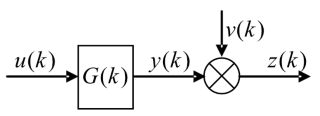
\includegraphics[width=.4\textwidth]{figure/增广最小二乘算法原理图.png} 
    \caption{SISO系统灰箱结构} % caption是图片的标题
    % \label{img} % 此处的label相当于一个图片的专属标志,目的是方便上下文的引用
\end{figure}
\noindent 其中,$y(k),\ z(k)$可表示为:
\begin{equation*}
    y(k) = -\sum_{i=1}^na_iy(k-i) + \sum_{i=1}^nb_iu(k-i)
\end{equation*}
\begin{equation*}
    z(k) = -\sum_{i=1}^na_iz(k-i) + \sum_{i=1}^nb_iu(k-i) + v(k) + \sum_{i=1}^nc_iv(k-i)
\end{equation*}
其中$v(k)$为非白噪声序列。定义以下变量:
\begin{align*}
    h(k) &= [-z(k-1),\ -z(k-2),\ \dots,\ -z(k-n),\ u(k-1),\ u(k-2),\ \\
    & \dots,\ u(k-n),\ \hat{v}(k-1),\ \dots,\ \hat{v}(k-n)]
\end{align*}
\begin{equation*}
    \theta = [a_1,\ a_2,\ \dots,\ a_n,\ b_1,\ b_2,\ \dots,\ b_n,\ c_1,\ \dots,\ c_n]^T
\end{equation*}
则$z(k)$也可以表示为:
\begin{equation*}
    z(k) = h(k)\theta + v(k)
\end{equation*}
类似于递推最小二乘算法,下面列出增广递推最小二乘算法的计算公式:
\begin{equation*}
    \hat{\theta}_{m+1} = \hat{\theta}_{m} + K_{m+1}[z(m+1) - h(m+1)\hat{\theta}_m]
\end{equation*}
\begin{equation*}
    P_{m+1} = P_m - P_m h^T(m+1)[w^{-1}(m+1) + h(m+1) P_m h^T(m+1)]^{-1} h(m+1) P_m
\end{equation*}
\begin{equation*}
    K_{m+1} = P_m h^T(m+1) [w^{-1}(m+1) + h(m+1) P_m h^T(m+1)]^{-1}
\end{equation*}

%
\section{实验对象和参数}
\paragraph{实验对象}
单输入-单输出系统,差分方程为:
% 无编号单行公式
\begin{equation*}
    z(k) + a_1z(k-1) + a_2z(k-2) = b_1u(k-1) + b_2u(k-2) + V(k)
\end{equation*}
\begin{equation*}
    V(k) = c_1v(k) + c_2v(k-1) + c_3v(k-2)
\end{equation*}

\paragraph{实验参数}
取真值:$a_1 = 1.6,\ a_2 = 0.7,\ b_1 = 1.0,\ b_2 = 0.4,\ c_1 = 1.1,\ c_2 = 1.4,\ c_3 = 0.3$,输入信号采用4阶M序列,幅值为1。$v(k)$的均值为0,方差分别为0.1和0.5的高斯噪声。

%
\section{程序框图}
%%
\subsection{一般最小二乘法程序框图}
\begin{figure}[H]
    \centering % 居中 
    % 图片文件的相对路径
    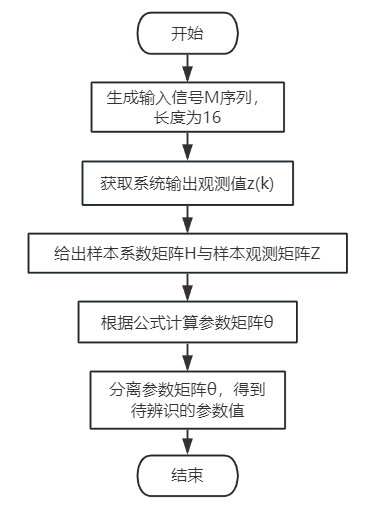
\includegraphics[width=.6\textwidth]{figure/一般最小二乘-流程图.png} 
    \caption{一般最小二乘法-程序框图} % caption是图片的标题
    % \label{img} % 此处的label相当于一个图片的专属标志,目的是方便上下文的引用
\end{figure}

%%
\subsection{递推最小二乘法程序框图}
\begin{figure}[H]
\centering
\begin{tikzpicture}[node distance=15pt]
    \node[draw, rounded corners] (start) {开始};
    \node[draw, below=of start] (step_1) {产生输入数据$u$和输出数据$z$};
    \node[draw, below=of step_1] (step_2) {初始化$P(0),\ \theta(0),\ w,\ \varepsilon$};
    \node[draw, below=of step_2] (step_3) {计算$P(k),\ \theta(k),\ K(k)$};
    \node[draw, diamond, aspect=4, below=of step_3, align=center] (choice_1) {$\forall i:\ \max | \frac{\hat{\theta}_i(k) - \hat{\theta}_i(k-1)}{\hat{\theta}_i(k-1)} | < \varepsilon?$};
    \node[draw, diamond, aspect=3, below=of choice_1, align=center] (choice_2) {$k > L?$};
    \node[draw, left=of choice_1, , text width=10em, align=center] (step_4) {$\theta(k-1) = \theta(k)$ $P(k-1) = P(k)$};
    \node[draw, rounded corners, below=of choice_2] (end) {结束};

    % dot
    \coordinate [right=15pt of choice_1] (dot_1) {};
    \coordinate [below=5pt of choice_2] (dot_2) {};

    \draw[->] (start) -- (step_1);
    \draw[->] (step_1) -- (step_2);
    \draw[->] (step_2) -- (step_3);
    \draw[->] (step_3) -- (choice_1);
    \draw[->] (choice_1) -- node[right]{否} (choice_2);
    \draw[->] (choice_2) -- node[left]{是} (end);

    \draw[->] (choice_2) -- node[above]{否} (choice_2-|step_4) -> (step_4);
    \draw[->] (step_4) -- (step_4|-step_3) -> (step_3);
    \draw[->] (choice_1) -- node[above]{是} (dot_1) -- (dot_1|-dot_2) -- (dot_2) -> (end);
\end{tikzpicture}
\caption{递推最小二乘法-程序框图}
\end{figure}

%%
\subsection{增广递推最小二乘法程序框图}
\begin{figure}[H]
    \centering % 居中 
    % 图片文件的相对路径
    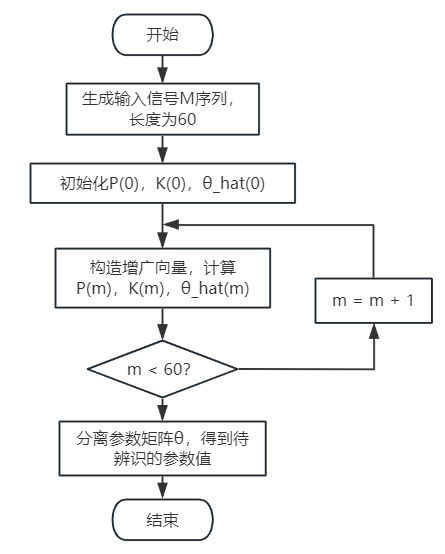
\includegraphics[width=.6\textwidth]{figure/增广递推最小二乘-程序框图.png} 
    \caption{增广递推最小二乘法-程序框图} % caption是图片的标题
    % \label{img} % 此处的label相当于一个图片的专属标志,目的是方便上下文的引用
\end{figure}

%
\section{程序代码}
\subsection{一般最小二乘法}
\begin{lstlisting}
% 一般最小二乘法
clear all
close all
clc

% 输入输出序列的长度
len = 16;
% 均值为0,方差为0.1的高斯噪声
v = normrnd(0, 0.1, 1, len);
% 均值为0,方差为0.5的高斯噪声
% v = normrnd(0, 0.5, 1, len);

%% M序列产生程序 4阶M序列 幅值为1
L = len; % M序列的周期
y1 = 1; y2 = 1; y3 = 1; y4 = 0; %四个移位积存器的输出初始值
for i = 1:L
    x1 = xor(y3, y4);
    x2 = y1;
    x3 = y2;
    x4 = y3;
    y(i) = y4;
    if y(i) > 0.5, u(i) = -1;
    else u(i) = 1;
    end
    y1 = x1; y2 = x2; y3 = x3; y4 = x4;
end
figure
stem(u), grid on
title('输入信号M序列')

%% 最小二乘辨识程序 
a1 = 1.6;
a2 = 0.7;
b1 = 1.0;
b2 = 0.4; 
c1 = 1.1;
c2 = 1.4;
c3 = 0.3;

z = zeros(1, len); %定义输出观测值的长度
for k = 3:16 
%     V(k) = c1*v(k) + c2*v(k-1) + c3*v(k-2);
    V(k) = v(k); %一般最小二乘用白噪声
    z(k) = -a1*z(k-1) - a2*z(k-2) + b1*u(k-1) + b2*u(k-2) + V(k);
end
figure(2)
plot([1:len], z)
title('输出观测值')
figure(3)
stem(z), grid on
title('输出观测值z的经线图形')

%% 参数辨识
%给样本系数矩阵
H=[-z(2) -z(1) u(2) u(1);-z(3) -z(2) u(3) u(2);
    -z(4) -z(3) u(4) u(3);-z(5) -z(4) u(5) u(4);
    -z(6) -z(5) u(6) u(5);-z(7) -z(6) u(7) u(6);
    -z(8) -z(7) u(8) u(7);-z(9) -z(8) u(9) u(8);
    -z(10) -z(9) u(10) u(9);-z(11) -z(10) u(11) u(10);
    -z(12) -z(11) u(12) u(11);-z(13) -z(12) u(13) u(12);
    -z(14) -z(13) u(14) u(13);-z(15) -z(14) u(15) u(14)];
%给出样本观测矩阵
Z = [z(3); z(4); z(5); z(6); z(7); z(8); z(9); z(10); z(11); 
        z(12); z(13); z(14); z(15); z(16)];
%计算参数
c = inv(H'*H)*H'*Z;
%分离参数
a1 = c(1), a2 = c(2), b1 = c(3), b2 = c(4)    
\end{lstlisting}

\subsection{递推最小二乘法}
\begin{lstlisting}
% 递推最小二乘法
clear all
close all
clc
% %产生N(0,1)正态分布的随机噪声
% randn('seed',100);
% v=randn(1,60); 

% 输入输出序列的长度
len = 60;
% 均值为0,方差为0.1的高斯噪声
v = normrnd(0, 0.1, 1, len);
% 均值为0,方差为0.5的高斯噪声
% v = normrnd(0, 0.5, 1, len);

%% M序列产生程序 4阶M序列 幅值为1
L = len - 1; % M序列的周期
y1 = 1; y2 = 1; y3 = 1; y4 = 0; %四个移位积存器的输出初始值
for i = 1:L
    x1 = xor(y3, y4);
    x2 = y1;
    x3 = y2;
    x4 = y3;
    y(i) = y4;
    if y(i) > 0.5, u(i) = -1;
    else u(i) = 1;
    end
    y1 = x1; y2 = x2; y3 = x3; y4 = x4;
end
figure
stem(u), grid on
title('输入信号M序列')

%% 一般递推最小二乘辨识程序
a1 = 1.6;
a2 = 0.7;
b1 = 1.0;
b2 = 0.4;
c1 = 1.1;
c2 = 1.4;
c3 = 0.3;

z = zeros(1, len); %定义输出观测值的长度
for k = 3:len 
%     V(k) = c1*v(k) + c2*v(k-1) + c3*v(k-2); % 有色噪声
    V(k) = v(k)
    z(k) = -a1*z(k-1) - a2*z(k-2) + b1*u(k-1) + b2*u(k-2) + V(k);
end
figure(2)
plot([1:len], z)
title('输出观测值')
figure(3)
stem(z), grid on
title('输出观测值z的经线图形')

%% 递推最小二乘辨识
c0 = [0.001 0.001 0.001 0.001]';
p0 = 10^3 * eye(4, 4);
E = 0.000000005; %相对误差
c = [c0, zeros(4, len - 1)]; %被辨识参数矩阵的初始值及大小
e = zeros(4, len); %相对误差的初始值及大小
lamt = 1;
% 迭代至k=16
for k = 3:len
    h1 = [-z(k-1), -z(k-2), u(k-1), u(k-2)]';
    k1 = p0 * h1 * inv(h1'*p0*h1 + 1*lamt);%求出K的值
    new = z(k) - h1'*c0; 
    c1 = c0 + k1*new;%求被辨识参数c
    p1 = 1/lamt*(eye(4) - k1*h1')*p0;
    e1 = (c1 - c0)./c0;%求参数当前值与上一次的值的差值
    e(:, k) = e1; %把当前相对变化的列向量加入误差矩阵的最后一列    
    c(:, k) = c1;%把辨识参数c 列向量加入辨识参数矩阵的最后一列 
    c0 = c1;%新获得的参数作为下一次递推的旧参数
    p0 = p1;
    if norm(e1) <= E 
        break; %若参数收敛满足要求,终止计算
    end
end
%分离参数
a1 = c(1, :);  a2 = c(2, :); b1 = c(3, :); b2 = c(4, :); 
ea1 = e(1, :); ea2 = e(2, :); eb1 = e(3, :); eb2 = e(4, :); 

figure(2);
i = 1:len;
%画出辨识结果
plot(i, a1, 'k', i, a2, 'b', i, b1, 'r', i, b2, 'g') 
legend('a1', 'a2', 'b1', 'b2');
title('递推最小二乘参数辨识')

figure(3); 
i = 1:len; 
%画出辨识结果的收敛情况
plot(i, ea1, 'k', i, ea2, 'b', i, eb1, 'r', i, eb2, 'g') 
legend('a1', 'a2', 'b1','b2');
title('辨识精度')
\end{lstlisting}

\subsection{增广最小二乘法}
\begin{lstlisting}
% 增广最小二乘法
clear all
close all
clc
% 输入输出序列的长度
len = 60;
% 均值为0,方差为0.1的高斯噪声
% v = normrnd(0, 0.1, 1, len);
% 均值为0,方差为0.5的高斯噪声
v = normrnd(0, 0.5, 1, len);

%% M序列、噪声信号产生及其显示程序 
L = 60;%四位移位积存器产生的M序列的周期
y1 = 1; y2 = 1; y3 = 1; y4 = 0;
for i = 1:L
    x1 = xor(y3, y4);
    x2 = y1;
    x3 = y2;
    x4 = y3;
    y(i) = y4;
    if y(i) > 0.5, u(i) = -1;
    else u(i) = 1;
    end
    y1 = x1; y2 = x2; y3 = x3; y4 = x4;
end
%画出M序列输入信号
figure(1);
stem(u),grid on

%% 增广递推最小二乘辨识
a1 = 1.6;
a2 = 0.7;
b1 = 1.0;
b2 = 0.4; 
c1 = 1.1;
c2 = 1.4;
c3 = 0.3;
z(2) = 0; z(1) = 0;
%直接给出被辨识参数的初始值,即一个充分小的实向量
theat0 = [0.001 0.001 0.001 0.001 0.001 0.001 0.001]';
p0 = 10^4 * eye(7, 7);%初始状态P0
theat = [theat0, zeros(7, len - 1)];%被辨识参数矩阵的初始值及大小
for k = 3:len 
    V(k) = c1*v(k) + c2*v(k-1) + c3*v(k-2);
    z(k) = -a1*z(k-1) - a2*z(k-2) + b1*u(k-1) + b2*u(k-2) + V(k);

    h1 = [-z(k-1), -z(k-2), u(k-1), u(k-2), ... 
                     v(k), v(k-1), v(k-2)]';
    x = h1'*p0*h1 + 1;
    x1 = inv(x); 
    k1 = p0*h1*x1; %K
    d1 = z(k) - h1'*theat0; 
    theat1 = theat0 + k1*d1;%辨识参数c 
    theat0 = theat1;%给下一次用
    theat(:, k) = theat1;%把辨识参数c 列向量加入辨识参数矩阵 
    p1 = p0 - k1*k1'*[h1'*p0*h1 + 1];%find p(k)
    p0 = p1; %给下次用
end%循环结束

%分离变量
a1v = theat(1, :);  a2v = theat(2, :); 
b1v = theat(3, :); b2v = theat(4, :);
c1v = theat(5, :); c2v = theat(6, :); c3v = theat(7, :); 
i = 1:60;    

% 输出
figure(2);
plot(i, z)

figure(3)
%参数估计值
plot(i, a1v, 'r', i, a2v, 'b', i, b1v, 'k', i, b2v, 'y', ... 
                    i, c1v, 'g', i, c2v, 'c', i, c3v, 'm')
legend('a1v', 'a2v', 'b1v', 'b2v', 'c1v', 'c2v', 'c3v');
title('参数估计值') %标题

% 参数估计误差
a1e = a1 - a1v;
a2e = a2 - a2v;
b1e = b1 - b1v;
b2e = b2 - b2v;
c1e = c1 - c1v;
c2e = c2 - c2v;
c3e = c3 - c3v;
figure(4)
plot(i, a1e, 'r', i, a2e, 'b', i, b1e, 'k', i, b2e, 'y', i,...
                         c1e, 'g', i, c2e, 'c', i, c3e, 'm')
legend('a1e', 'a2e', 'b1e', 'b2e', 'c1e', 'c2e', 'c3e');
title('参数估计误差') %标题      
\end{lstlisting}

%
\section{实验结果及分析}
采用均值为0,方差分别为0.1和0.5的高斯噪声,比较实验结果。

%%
\subsection{一般最小二乘法}
%%%
\paragraph{高斯噪声:均值为0,方差为0.1}~{}

采用四阶M序列作为系统输入,幅值为1,长度为16:
\begin{figure}[H]
    \centering % 居中 
    % 图片文件的相对路径
    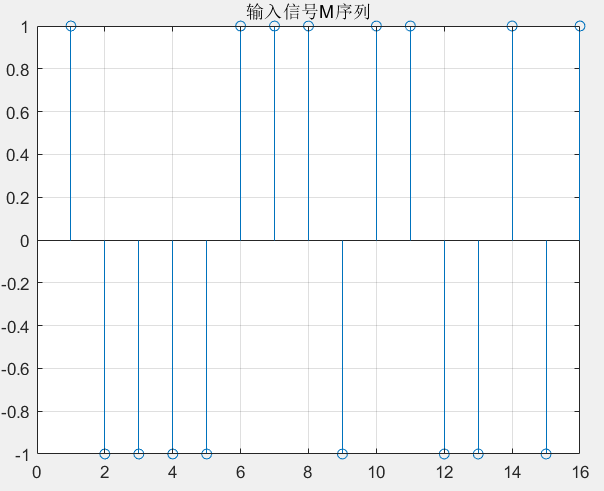
\includegraphics[width=.8\textwidth]{figure/一般最小二乘-输入信号M序列.png} 
    \caption{一般最小二乘-输入信号M序列} % caption是图片的标题
    % \label{img} % 此处的label相当于一个图片的专属标志,目的是方便上下文的引用
\end{figure}

系统的输出观测值如下图所示:
\begin{figure}[H]
    \centering % 居中 
    % 图片文件的相对路径
    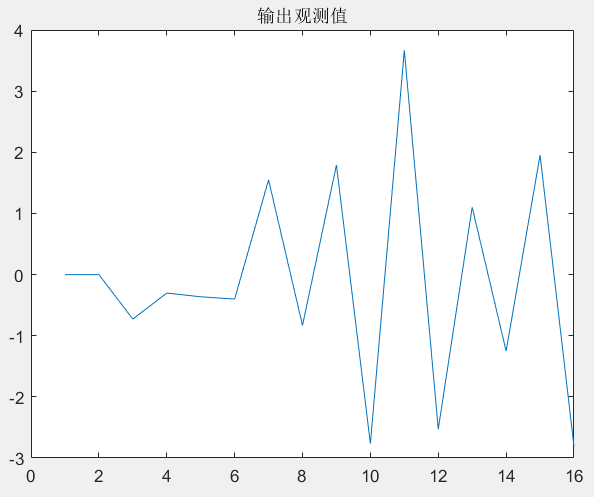
\includegraphics[width=.8\textwidth]{figure/一般最小二乘-输出观测值.png} 
    \caption{一般最小二乘-输出观测值(噪声方差:0.1)} % caption是图片的标题
    % \label{img} % 此处的label相当于一个图片的专属标志,目的是方便上下文的引用
\end{figure}
\begin{figure}[H]
    \centering % 居中 
    % 图片文件的相对路径
    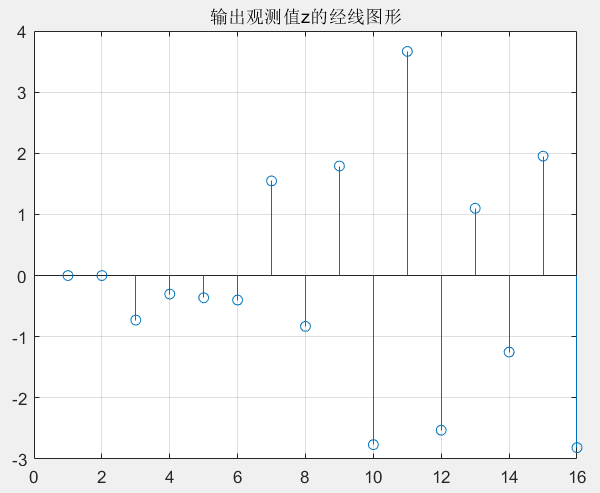
\includegraphics[width=.8\textwidth]{figure/一般最小二乘-输出观测值的经线图形.png} 
    \caption{一般最小二乘-输出观测值的经线图形(噪声方差:0.1)} % caption是图片的标题
    % \label{img} % 此处的label相当于一个图片的专属标志,目的是方便上下文的引用
\end{figure}

最终的参数辨识结果如下:
\begin{table}[H]
\centering % 居中
\begin{tabular}{cccc} % 指明列数
    \toprule % 顶部粗线
    辨识参数 & 实际值 & 辨识值 & 误差百分比(\%) \\
    \midrule % 中间细线
    $a_1$ & 1.6 & 1.6346 & 2.16 \\
    $a_2$ & 0.7 & 0.7463 & 6.61 \\
    $b_1$ & 1.0 & 0.9733 & 2.67 \\
    $b_2$ & 0.4 & 0.4069 & 1.72 \\
    \bottomrule % 底部粗线
\end{tabular}
\caption{一般最小二乘法辨识结果(噪声方差:0.1)} % 标题
\end{table}

\paragraph{结果分析}~{}

由于噪声项产生的随机性,每次运行程序所得结果均有不同。由实验结果可以看出,本次参数辨识的误差百分比基本在$\pm 5\%$以内,说明在噪声方差为0.1的条件下,采用一般最小二乘法进行参数辨识的结果是相对可靠的。


%%%
\paragraph{高斯噪声:均值为0,方差为0.5}~{}

采用四阶M序列作为系统输入,幅值为1,长度为16,同上。系统的输出观测值如下图所示:
\begin{figure}[H]
    \centering % 居中 
    % 图片文件的相对路径
    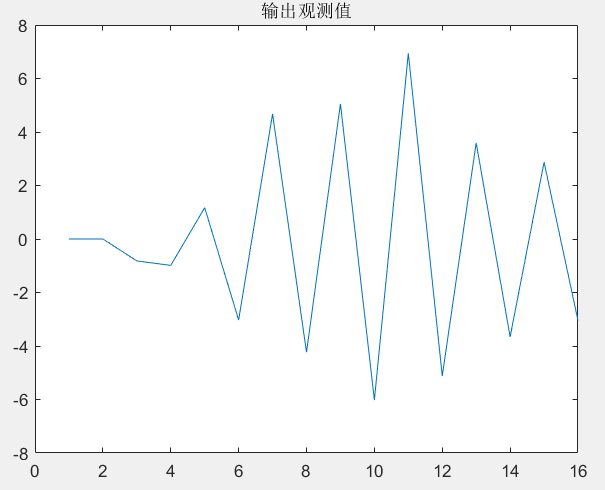
\includegraphics[width=.8\textwidth]{figure/一般最小二乘-输出观测值(噪声方差0.5).png} 
    \caption{一般最小二乘-输出观测值(噪声方差0.5)} % caption是图片的标题
    % \label{img} % 此处的label相当于一个图片的专属标志,目的是方便上下文的引用
\end{figure}
\begin{figure}[H]
    \centering % 居中 
    % 图片文件的相对路径
    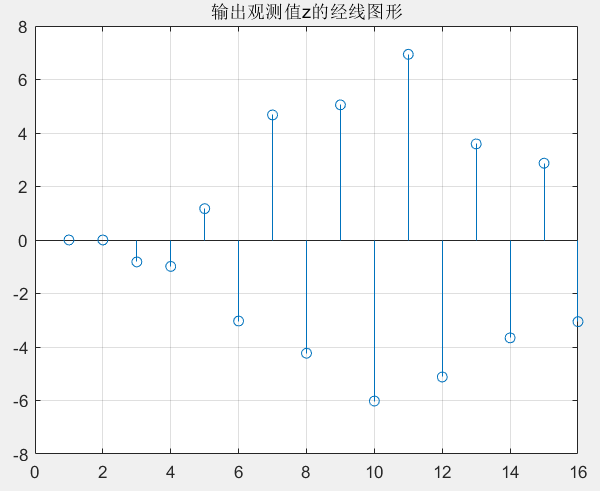
\includegraphics[width=.8\textwidth]{figure/一般最小二乘-输出观测值的经线图形(噪声方差0.5).png} 
    \caption{一般最小二乘-输出观测值的经线图形(噪声方差0.5)} % caption是图片的标题
    % \label{img} % 此处的label相当于一个图片的专属标志,目的是方便上下文的引用
\end{figure}

最终的参数辨识结果如下:
\begin{table}[H]
\centering % 居中
\begin{tabular}{cccc} % 指明列数
    \toprule % 顶部粗线
    辨识参数 & 实际值 & 辨识值 & 误差百分比(\%) \\
    \midrule % 中间细线
    $a_1$ & 1.6 & 1.4706 & 8.09 \\
    $a_2$ & 0.7 & 0.5299 & 24.3 \\
    $b_1$ & 1.0 & 1.0543 & 5.43 \\
    $b_2$ & 0.4 & 0.3322 & 16.95 \\
    \bottomrule % 底部粗线
\end{tabular}
\caption{一般最小二乘法辨识结果(噪声方差:0.5)} % 标题
\end{table}

\paragraph{结果分析}~{}

对比噪声方差为0.1的实验结果可以看出,当噪声方差增大时,使用一般最小二乘法辨识参数的结果出现了较大的误差。因此在这种条件下,一般最小二乘参数辨识方法不再适用。

%%
\subsection{递推最小二乘法}
%%%
\paragraph{高斯噪声:均值为0,方差为0.1}~{}

采用M序列作为系统输入,幅值为1,长度为60:
\begin{figure}[H]
    \centering % 居中 
    % 图片文件的相对路径
    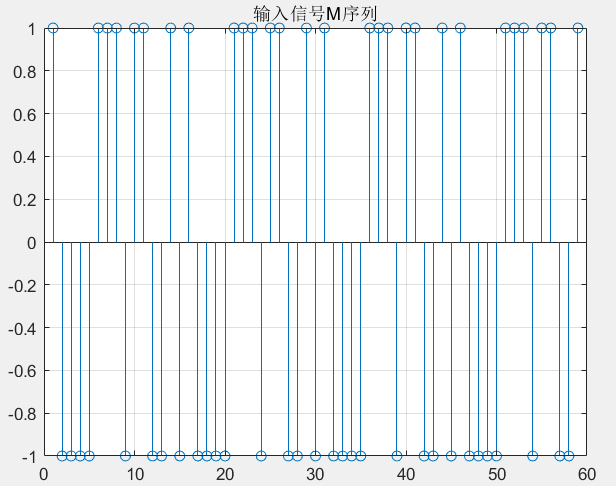
\includegraphics[width=.8\textwidth]{figure/递推最小二乘-输入信号M序列.png} 
    \caption{递推最小二乘-输入信号M序列} % caption是图片的标题
    % \label{img} % 此处的label相当于一个图片的专属标志,目的是方便上下文的引用
\end{figure}

迭代过程中参数辨识值及辨识精度如下图所示:
\begin{figure}[H]
    \centering % 居中 
    % 图片文件的相对路径
    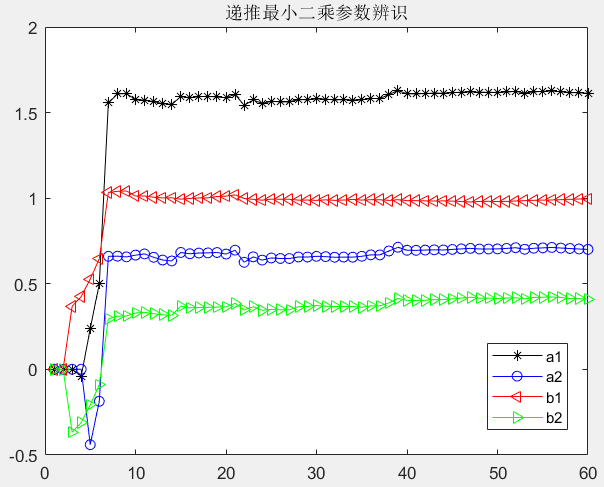
\includegraphics[width=.8\textwidth]{figure/递推最小二乘-参数辨识结果.png} 
    \caption{递推最小二乘-参数辨识结果(噪声方差0.1)} % caption是图片的标题
    % \label{img} % 此处的label相当于一个图片的专属标志,目的是方便上下文的引用
\end{figure}
\begin{figure}[H]
    \centering % 居中 
    % 图片文件的相对路径
    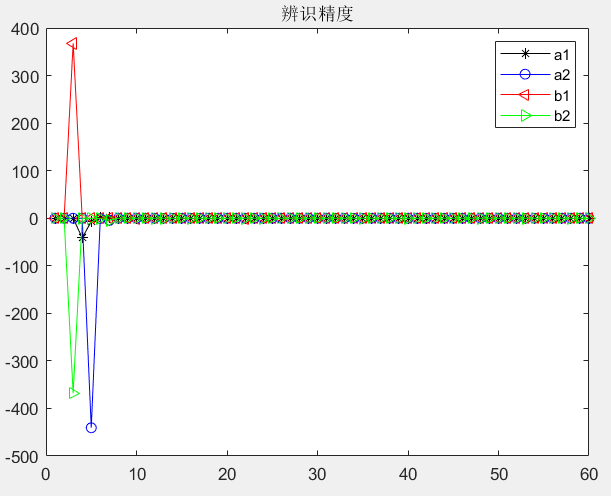
\includegraphics[width=.8\textwidth]{figure/递推最小二乘-辨识精度.png} 
    \caption{递推最小二乘-辨识精度(噪声方差0.1)} % caption是图片的标题
    % \label{img} % 此处的label相当于一个图片的专属标志,目的是方便上下文的引用
\end{figure}

最终的参数辨识结果如下:
\begin{table}[H]
\centering % 居中
\begin{tabular}{cccc} % 指明列数
    \toprule % 顶部粗线
    辨识参数 & 实际值 & 辨识值 & 误差百分比(\%) \\
    \midrule % 中间细线
    $a_1$ & 1.6 & 1.6163 & 1.02 \\
    $a_2$ & 0.7 & 0.7129 & 0.0184 \\
    $b_1$ & 1.0 & 1.0003 & 0.03 \\
    $b_2$ & 0.4 & 0.4245 & 6.12 \\
    \bottomrule % 底部粗线
\end{tabular}
\caption{递推最小二乘法辨识结果(噪声方差:0.1)} % 标题
\end{table}

%%%
\paragraph{高斯噪声:均值为0,方差为0.5}~{}

采用M序列作为系统输入,幅值为1,长度为60,同上。迭代过程中参数辨识值及辨识精度如下图所示:
\begin{figure}[H]
    \centering % 居中 
    % 图片文件的相对路径
    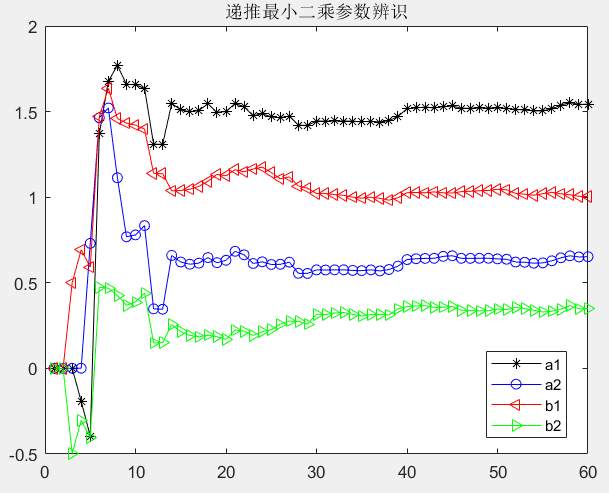
\includegraphics[width=.8\textwidth]{figure/递推最小二乘-参数辨识结果(方差0.5).png} 
    \caption{递推最小二乘-参数辨识结果(噪声方差0.5)} % caption是图片的标题
    % \label{img} % 此处的label相当于一个图片的专属标志,目的是方便上下文的引用
\end{figure}
\begin{figure}[H]
    \centering % 居中 
    % 图片文件的相对路径
    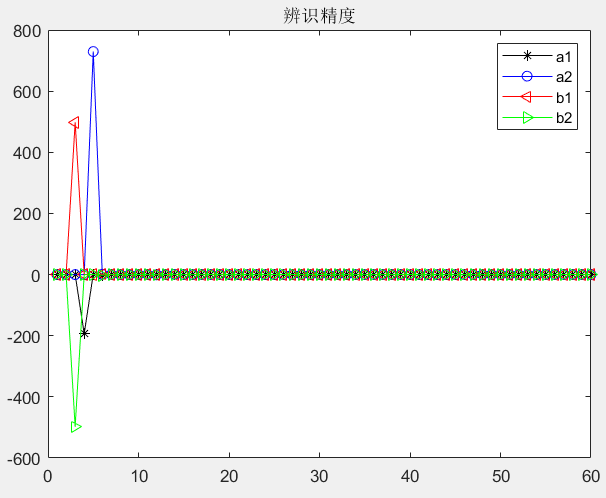
\includegraphics[width=.8\textwidth]{figure/递推最小二乘-辨识精度(方差0.5).png} 
    \caption{递推最小二乘-辨识精度(噪声方差0.5)} % caption是图片的标题
    % \label{img} % 此处的label相当于一个图片的专属标志,目的是方便上下文的引用
\end{figure}

最终的参数辨识结果如下:
\begin{table}[H]
\centering % 居中
\begin{tabular}{cccc} % 指明列数
    \toprule % 顶部粗线
    辨识参数 & 实际值 & 辨识值 & 误差百分比(\%) \\
    \midrule % 中间细线
    $a_1$ & 1.6 & 1.3634 & 14.79 \\
    $a_2$ & 0.7 & 0.4394 & 0.3723 \\
    $b_1$ & 1.0 & 0.9314 & 6.86 \\
    $b_2$ & 0.4 & 0.2035 & 49.13 \\
    \bottomrule % 底部粗线
\end{tabular}
\caption{递推最小二乘法辨识结果(噪声方差:0.5)} % 标题
\end{table}

\paragraph{结果分析}~{}

与一般最小二乘参数辨识方法的实验结果类似,当噪声方差较小(0.1)时,递推最小二乘参数辨识方法的参数估计误差大致在$\pm 5\%$以内;而当噪声方差较大(0.5)时,最终的参数估计值出现了很大的误差。实验结果说明在噪声干扰较大的情况下,使用递推最小二乘方法进行参数辨识就不再适用了。

另外需要指出的是,一般最小二乘和递推最小二乘参数辨识方法均无法对噪声项参数进行辨识,这是两种方法在适用性上存在的另一局限性。

%%
\subsection{增广递推最小二乘法}
%%%
\paragraph{高斯噪声:均值为0,方差为0.1}~{}

采用M序列作为系统输入,幅值为1,长度为60:
\begin{figure}[H]
    \centering % 居中 
    % 图片文件的相对路径
    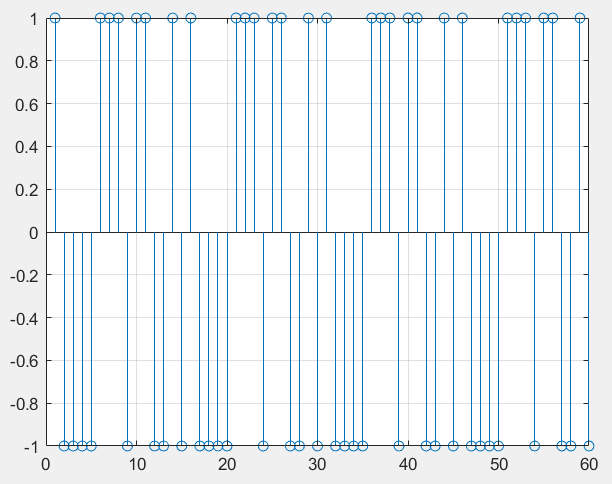
\includegraphics[width=.8\textwidth]{figure/增广递推最小二乘-输入信号M序列.png} 
    \caption{增广递推最小二乘-输入信号M序列} % caption是图片的标题
    % \label{img} % 此处的label相当于一个图片的专属标志,目的是方便上下文的引用
\end{figure}

迭代过程中的参数估计值及估计误差如下图所示:
\begin{figure}[H]
    \centering % 居中 
    % 图片文件的相对路径
    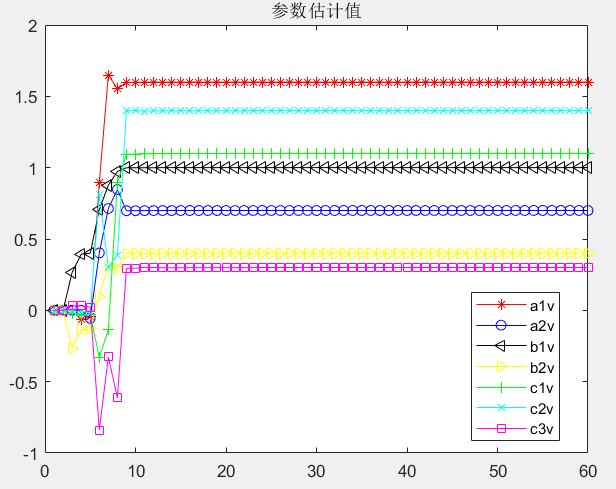
\includegraphics[width=.8\textwidth]{figure/增广递推最小二乘-参数估计值.png} 
    \caption{增广递推最小二乘-参数估计值(噪声方差0.1)} % caption是图片的标题
    % \label{img} % 此处的label相当于一个图片的专属标志,目的是方便上下文的引用
\end{figure}
\begin{figure}[H]
    \centering % 居中 
    % 图片文件的相对路径
    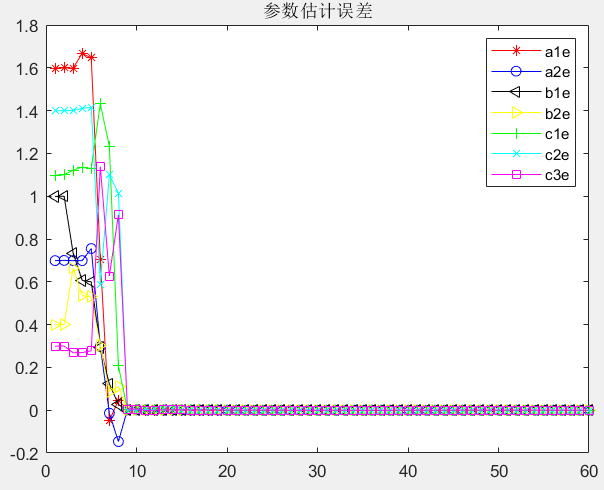
\includegraphics[width=.8\textwidth]{figure/增广递推最小二乘-参数估计误差.png} 
    \caption{增广递推最小二乘-参数估计误差(噪声方差0.1)} % caption是图片的标题
    % \label{img} % 此处的label相当于一个图片的专属标志,目的是方便上下文的引用
\end{figure}

最终的参数辨识结果如下:
\begin{table}[H]
\centering % 居中
\begin{tabular}{cccc} % 指明列数
    \toprule % 顶部粗线
    辨识参数 & 实际值 & 辨识值 & 误差百分比(\%) \\
    \midrule % 中间细线
    $a_1$ & 1.6 & 1.59996 & 0.0025 \\
    $a_2$ & 0.7 & 0.699968 & 0.0046 \\
    $b_1$ & 1.0 & 0.999994 & 0.0006 \\
    $b_2$ & 0.4 & 0.399967 & 0.0083 \\
    $c_1$ & 1.1 & 1.0998 & 0.0182 \\
    $c_2$ & 1.4 & 1.39968 & 0.0229 \\
    $c_3$ & 0.3 & 0.299943 & 0.019 \\
    \bottomrule % 底部粗线
\end{tabular}
\caption{增广递推最小二乘法辨识结果(噪声方差:0.1)} % 标题
\end{table}

%%%
\paragraph{高斯噪声:均值为0,方差为0.5}~{}

采用M序列作为系统输入,幅值为1,长度为60,同上。迭代过程中的参数估计值及估计误差如下图所示:
\begin{figure}[H]
    \centering % 居中 
    % 图片文件的相对路径
    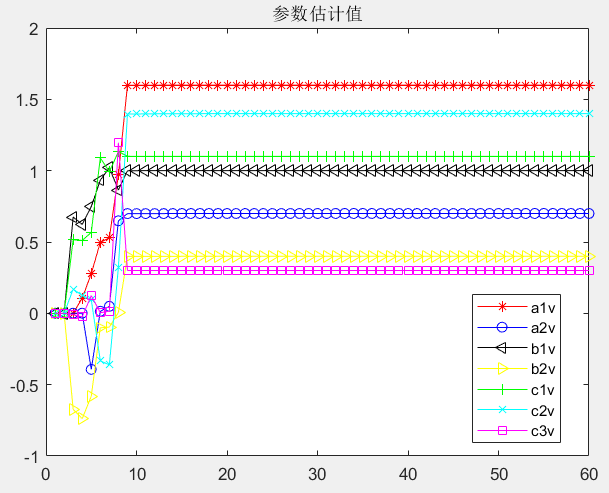
\includegraphics[width=.8\textwidth]{figure/增广递推最小二乘-参数估计值(方差0.5).png} 
    \caption{增广递推最小二乘-参数估计值(噪声方差0.5)} % caption是图片的标题
    % \label{img} % 此处的label相当于一个图片的专属标志,目的是方便上下文的引用
\end{figure}
\begin{figure}[H]
    \centering % 居中 
    % 图片文件的相对路径
    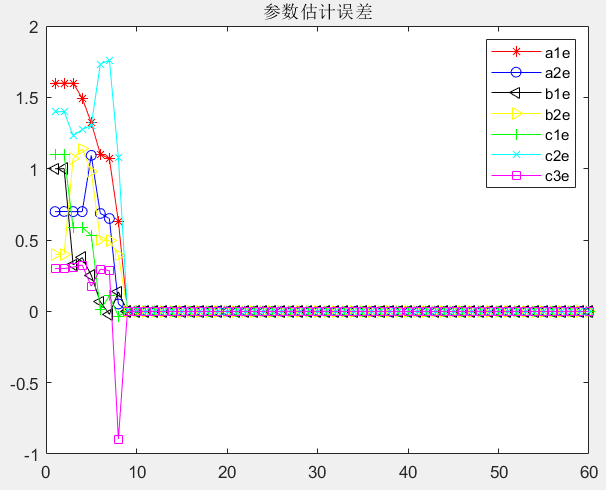
\includegraphics[width=.8\textwidth]{figure/增广递推最小二乘-参数估计误差(方差0.5).png} 
    \caption{增广递推最小二乘-参数估计误差(噪声方差0.5)} % caption是图片的标题
    % \label{img} % 此处的label相当于一个图片的专属标志,目的是方便上下文的引用
\end{figure}

最终的参数辨识结果如下:
\begin{table}[H]
\centering % 居中
\begin{tabular}{cccc} % 指明列数
    \toprule % 顶部粗线
    辨识参数 & 实际值 & 辨识值 & 误差百分比(\%) \\
    \midrule % 中间细线
    $a_1$ & 1.6 & 1.59997 & 0.0019 \\
    $a_2$ & 0.7 & 0.69997 & 0.0043 \\
    $b_1$ & 1.0 & 0.999996 & 0.0004 \\
    $b_2$ & 0.4 & 0.399968 & 0.0080 \\
    $c_1$ & 1.1 & 1.09999 & 0.0009 \\
    $c_2$ & 1.4 & 1.39996 & 0.0029 \\
    $c_3$ & 0.3 & 0.299979 & 0.0070 \\
    \bottomrule % 底部粗线
\end{tabular}
\caption{增广递推最小二乘法辨识结果(噪声方差:0.5)} % 标题
\end{table}

\paragraph{结果分析}~{}

对比前述两种最小二乘参数辨识方法,基于增广递推的参数辨识方法的辨识效果明显更好。通过参数估计值的变化情况可以看出,增广递推的收敛速度更快,参数估计值的波动更小;而且在相同的迭代次数下,增广递推得到的参数辨识结果的精度显著高于前述两种辨识方法;此外,在噪声干扰较大的条件下,增广递推参数辨识方法也有非常好的表现;最后值得指出的一点是,增广递推还可以对噪声项参数进行辨识,这使得增广递推参数辨识方法拥有更广的适用范围。

%
\section{结论}
根据以上实验结果可以得出,在弱噪声干扰情况下,使用一般最小二乘、递推最小二乘和增广递推最小二乘的参数辨识方法均能取得不错的效果,具有较高的可靠性;而在强噪声干扰情况下,一般最小二乘和递推最小二乘参数辨识方法则会出现较大的偏差,不再适用,而增广最小二乘参数辨识方法不会受到明显的影响,参数辨识精度始终能保持在较高的水平。此外,相比一般最小二乘和递推最小二乘参数辨识方法,增广递推最小二乘参数辨识方法还可以针对噪声项参数进行辨识,且辨识精度很高。综上所述,在参数辨识的可靠性和辨识精度方面,增广递推最小二乘辨识方法是最优的,其他两种参数辨识方法效果相对较差。


%%%%%%%%%%%%%%%%%%%%%%%%%%%%%%%%%%%%%%%%%%%%%%%%%%%%%%%%%%%%%%
% 极大似然方法估计参数值
\begin{titlepage}
% 封面信息
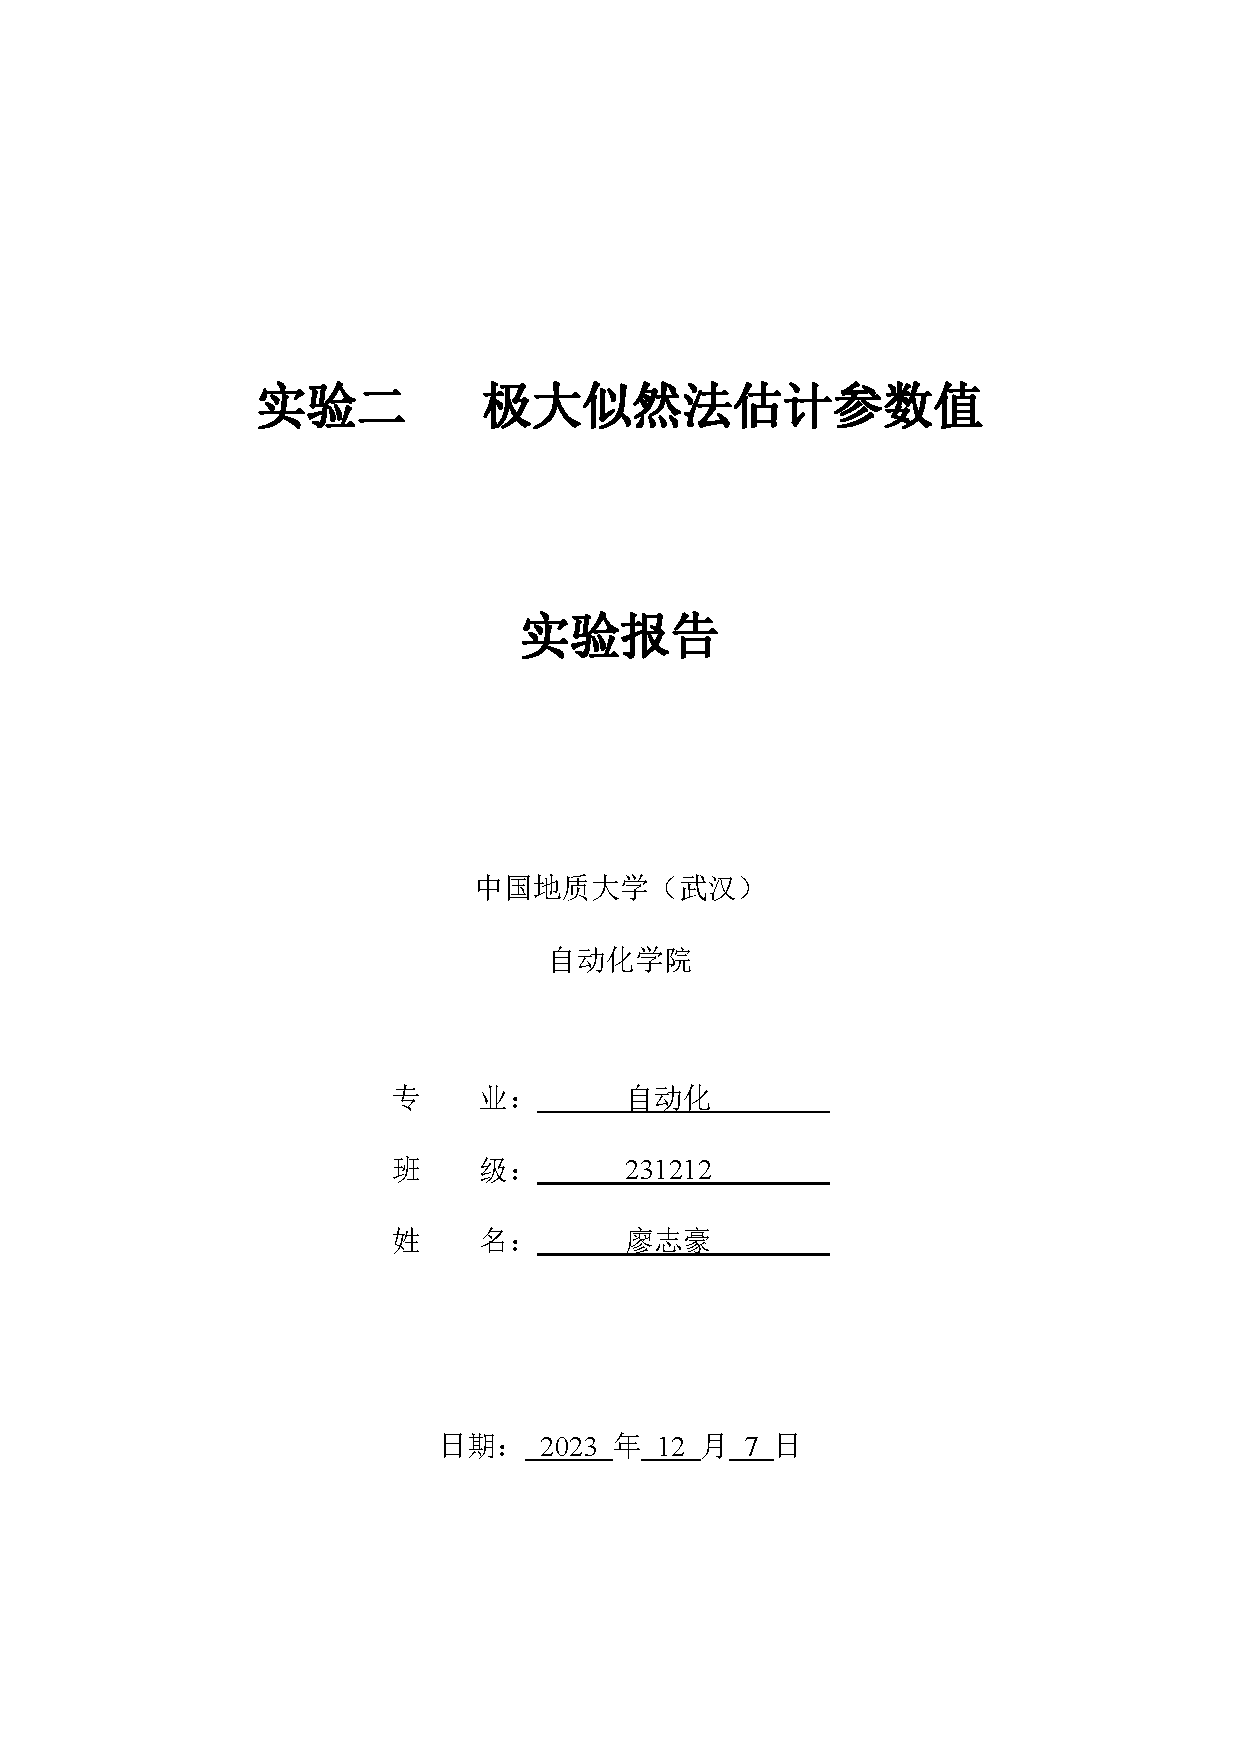
\includepdf[pages={1}]{cover/实验二封面.pdf}
\end{titlepage}
% 重置章节编号
\setcounter{section}{0}
%
\section{实验题目}
设系统动态模型为:
\begin{equation*}
    y(k) + a_1y(k-1) + a_2y(k-2) = b_1u(k-1) + b_2u(k-2) + \varepsilon(k) + d_1\varepsilon(k-1) + d_2\varepsilon(k-2)
\end{equation*}

其中模型参数:$a_1 = -0.5,\ a_2 = -0.2,\ b_1 = 1.0,\ b_2 = 1.5, d_1 = -0.8,\ d_2 = 0.3$,噪声$\varepsilon(k)$是均值为零,方差为0.01的高斯白噪声,$u(k)$是由4级移位寄存器产生的幅度为1的M序列,利用极大似然参数估计递推算法对系统参数进行辨识。


%
\section{实验目的}
\begin{enumerate}
    \item 掌握极大似然法估计参数值的原理;
    \item 掌握极大似然法的 Matlab 实现和估计参数的编程;
    \item 分析极大似然法的优缺点、理解极大似然法辨识的物理意义。
\end{enumerate}


%
\section{实验主要原理}
%%
\subsection{极大似然参数估计原理}
设离散随机过程${Y_k}$与未知参数$\theta$有关,假定已知概率分布密度函数$f(Y_k|\theta)$。如果我们得到$n$个独立的观测值:$Y_1,\ Y_2,\ …,\ Y_n$,则可得概率密度分布分别为:$f(Y_1|\theta),\ f(Y_2|\theta),\ …,$ $\ f(Y_n|\theta)$。要求根据这些观测值来估计未知参数$\theta$,估计的准则是使得观测值${Y_k}$的出现概率为最大。为此,定义一个似然函数:
\begin{equation*}
    L(Y_1,\ Y_2,\ \dots,\ Y_N|\theta) = f(Y_1|\theta)f(Y_2|\theta)\dots(Y_N|\theta)
\end{equation*}

上式的右边是$n$个概率密度函数的连乘,似然函数$L$是$\theta$的函数。如果$L$达到最大值,则${Y_k}$出现的概率为最大。因此极大似然法的实质就是求出使得$L$达到极大值的$\theta$的估值。对上式取对数并求偏导即可得到$\theta$的极大似然估计:
\begin{equation*}
    \hat{\theta}_{ML} = \frac{1}{N}\sum_{i=1}^Ny_i
\end{equation*}

极大似然法辨识的物理意义:根据一组确定的随机序列$Y_N$,设法找到参数估计值$\hat{\theta}_{ML}$,它使得随机变量$y$在$\hat{\theta}_{ML}$条件下的概率密度函数最大可能地逼近随机变量$y$在$\theta$(真值)条件下的概率密度函数,即:
\begin{equation*}
    p(y|\hat{\theta}_{ML}) \stackrel{max}{--\rightarrow} p(y|\theta)
\end{equation*}

%%
\subsection{Newton-Raphson方法原理}
\paragraph{Newton-Raphson方法的思想}~{}

根据第L次迭代得到的参数估计$\hat{\theta}(L),\ \hat{\theta}(L + 1)$:
\begin{equation*}
    J_{L + 1}(\hat{\theta}(L + 1)) \le J_L(\hat{\theta}(L)) 
\end{equation*}
其中:
\begin{equation*}
    J_L(\theta) = \frac{1}{2}\sum_{k = (L - 1)N + n + 1}^{NL + n}\varepsilon^2(k) 
\end{equation*}


\paragraph{Newton-Raphson法应用于极大似然参数估计}~{}

Newton-Raphson法应用于极大似然估计求解的步骤:
\begin{enumerate}
    \item 确定初始值$\hat{\theta}_0$
    
    先采集一批输入输出数据$\{ y(k) \},\ \{ u(k) \}$,用最小二乘法获得$\hat{a}_1, ..., \hat{a}_n,$ $\hat{b}_1, ..., \hat{b}_n$,对于$\hat{\theta}(L)$中的$\hat{d}_1, ..., \hat{d}_n$,可先任意假定初值。

    \item 设定初始$\varepsilon(1), \varepsilon(2), ..., \varepsilon(n)$和$\frac{\partial\varepsilon(1)}{\partial\theta}|_{\theta = \hat{\theta}(L)},\frac{\partial\varepsilon(2)}{\partial\theta}|_{\theta = \hat{\theta}(L)}, ..., \frac{\partial\varepsilon(n)}{\partial\theta}|_{\theta = \hat{\theta}(L)}$,为方便起见,通常均取零。
    
    \item 计算$\varepsilon(k)$
    
    采集一批长度为N的数据$\{ y(k) \}, \{ u(k) \}$,利用$\hat{\theta}(L)$和$\varepsilon(k)$,根据下式计算新的$\varepsilon(k)(k = NL + n + 1, NL + n + 2, ..., NL + n + N)$:
    \begin{equation*}
        \varepsilon(k) = y(k) + \sum_{i = 1}^n \hat{a}_iy(k - i) - \sum_{i = 1}^n \hat{b}_iu(k - i) - \sum_{i = 1}^n \hat{d}_i\varepsilon(k - i)
    \end{equation*}

    \item 计算$\frac{\partial \varepsilon(k)}{\partial \theta}|_{\theta = \hat{\theta}(L)}(k = NL + n + 1, NL + n + 2, ..., NL + n + N)$
    
    根据下式计算$\frac{\partial \varepsilon(k)}{\partial \theta}|_{\theta = \hat{\theta}(L)}$:
    \begin{equation*}
        \frac{\partial\varepsilon(k)}{\partial a_j} = y(k - j) - \sum_{i = 1}^n d_i \frac{\partial \varepsilon(k - i)}{\partial a_j}|_{\theta = \hat{\theta}(L)} 
    \end{equation*}
    \begin{equation*}
        \frac{\partial \varepsilon(k)}{\partial b_j} = -u(k - j) - \sum_{i = 1}^n d_i \frac{\partial \varepsilon(k - i)}{\partial b_j}|_{\theta = \hat{\theta}(L)}
    \end{equation*}
    \begin{equation*}
        \frac{\partial \varepsilon(k)}{\partial d_j} = -\varepsilon(k - j) - \sum_{i = 1}^n d_i \frac{\partial \varepsilon(k - i)}{\partial d_j}|_{\theta = \hat{\theta}(L)}
    \end{equation*}

    \item 计算梯度阵$\frac{\partial J_{L + 1}}{\partial \theta}|_{\theta = \hat{\theta}(L)}$和$Hessian$阵$\frac{\partial^2 J_{L + 1}}{\partial (\theta)^2}|_{\theta = \hat{\theta}(L)}$
    
    利用所计算的$\varepsilon(k)$和$\frac{\partial \varepsilon(k)}{\partial \theta}|_{\theta = \hat{\theta}(L)}$:
    \begin{equation*}
        \frac{\partial J_{L + 1}}{\partial \theta}|_{\theta = \hat{\theta}(L)} = \sum_{k = NL + n + 1}^{(L + 1)N + n} \varepsilon(k) \cdot \frac{\partial \varepsilon(k)}{\partial \theta}|_{\theta = \hat{\theta}(L)} 
    \end{equation*}
    \begin{equation*}
        \frac{\partial^2 J_{L + 1}}{\partial (\theta)^2}|_{\theta = \hat{\theta}(L)} \approx \sum_{k = NL + n + 1}^{(L + 1)N + n}\frac{\partial \varepsilon(k)}{\partial \theta}[\frac{\partial \varepsilon(k)}{\partial \theta}]^T|_{\theta = \hat{\theta}(L)}
    \end{equation*}

    \item 计算新的估值$\hat{\theta}(L + 1)$
    \begin{equation*}
        \hat{\theta}(L + 1) = \hat{\theta}(L) - [\frac{\partial^2 J_{L + 1}}{\partial (\theta)^2}]^{-1}|_{\theta = \hat{\theta}(L)} \cdot \frac{\partial J_{L + 1}}{\partial \theta}|_{\theta = \hat{\theta}(L)}
    \end{equation*}

    \item 取最后$n$个$\varepsilon(k)$和$\frac{\partial \varepsilon(k)}{\partial \theta}_{\theta = \hat{\theta}(L)}$值,作为下一次迭代的初值,$L = L + 1$,转到 $3.$ 继续循环,直至满足停止条件。设经过$r$次迭代计算后得到$\hat{\theta}(r)$,则停止迭代标准为:
    \begin{equation*}
        || \hat{\theta}(r + 1) - \hat{\theta}(r) || \le \Delta 
    \end{equation*}
    \begin{equation*}
        | \frac{\sigma_{r + 1}^2 - \sigma_r^2}{\sigma_r^2} | \le \nu, \quad r = M
    \end{equation*}
\end{enumerate}

\paragraph{说明}~{}
\begin{enumerate}
    \item 该数值算法即使当系统噪声水平较高时也能获得良好的估计
    \item 需要进行N次观测,才能进行一次递推
\end{enumerate}


%
\section{实验对象或参数}
\paragraph{实验对象}
系统动态模型为:
\begin{equation*}
    y(k) + a_1y(k-1) + a_2y(k-2) = b_1u(k-1) + b_2u(k-2) + \varepsilon(k) + d_1\varepsilon(k-1) + d_2\varepsilon(k-2)
\end{equation*}

\paragraph{实验参数}
模型参数:$a_1 = -0.5,\ a_2 = -0.2,\ b_1 = 1.0,\ b_2 = 1.5, d_1 = -0.8,\ d_2 = 0.3$,噪声$\varepsilon(k)$是均值为零,方差为0.01的高斯白噪声,$u(k)$是由4级移位寄存器产生的幅度为1的M序列。

%
\section{程序框图}
%%
\subsection{递推的极大似然参数估计}
\begin{figure}[H]
    \centering % 居中 
    % 图片文件的相对路径
    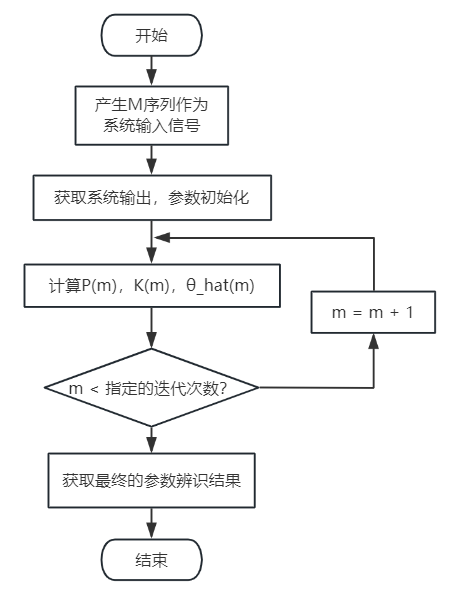
\includegraphics[width=.6\textwidth]{figure/递推极大似然-程序框图.png} 
    \caption{递推极大似然法-程序框图} % caption是图片的标题
    % \label{img} % 此处的label相当于一个图片的专属标志,目的是方便上下文的引用
\end{figure}

%%
\subsection{Newton-Raphson方法}
\begin{figure}[H]
\centering
\begin{tikzpicture}[node distance=15pt]
    \node[draw, rounded corners] (start) {开始};
    \node[draw, below=of start, text width=20em, align=center] (step_1) {设定初始估计值$\hat{\theta}(1),\ v(1),\ v(2),\ \dots,\ v(n)$和$\frac{\partial v(1)}{\partial\theta},\ \dots,\ \frac{\partial v(n)}{\partial\theta}$,并设置$j = 1$};
    \node[draw, below=of step_1] (step_2) {计算误差$v(n+1),\ v(n+2),\ \dots,\ v(n+N)$};
    \node[draw, below=of step_2] (step_3) {计算$\frac{\partial v(k)}{\partial \theta}|_{\theta = \hat{\theta}(j)}$};
    \node[draw, below=of step_3, text width=20em, align=center] (step_4) {计算梯度矩阵$\frac{\partial J(\theta)}{\partial \theta}|_{\theta = \hat{\theta}(j)}$和$Hessian$矩阵$\frac{\partial^2 J(\theta)}{(\partial \theta)^2}|_{\theta = \hat{\theta}(j)}$};
    \node[draw, below=of step_4, text width=20em, align=center] (step_5) {计算新的参数估计值$\hat{\theta}(j+1) = \hat{\theta}(j) - [\frac{\partial^2 J(\theta)}{(\partial \theta)^2}]^{-1}_{\theta = \hat{\theta}(j)} \cdot \frac{\partial J(\theta)}{\partial \theta}|_{\theta = \hat{\theta}(j)}$};
    \node[draw, diamond, aspect=3, below=of step_5, text width=10em, align=center] (choice) {是否满足迭代停止条件?};
    \node[draw, below=30pt of choice] (step_6) {取$n$个$v(k)$和$\frac{\partial v(k)}{\partial \theta}$作为下次迭代的初值};
    \node[draw, below=of step_6] (step_7) {$j = j + 1$};
    \node[draw, right=30pt of choice, text width=7em, align=center] (step_8) {输出$\hat{\theta}(j+1)$,停止计算};
    \node[draw, rounded corners, below=15pt of step_7]  (end) {结束};
    % dot
    \coordinate [below=5pt of step_7] (dot1) {};
    \coordinate [left=120pt of step_7] (dot2) {};

    \draw[->] (start) -- (step_1);
    \draw[->] (step_1) -- (step_2);
    \draw[->] (step_2) -- (step_3);
    \draw[->] (step_3) -- (step_4);
    \draw[->] (step_4) -- (step_5);
    \draw[->] (step_5) -- (choice);
    \draw[->] (choice) -- node[right] {否} (step_6);
    \draw[->] (step_6) -- (step_7);
    \draw[->] (choice) -- node[above] {是}  (step_8);
    \draw[->] (step_8) -- (step_8|-dot1) -- (dot1) -> (end);

    \draw[->] (step_7) -- (step_7-|dot2) -- (dot2|-step_2) -> (step_2);
\end{tikzpicture}
\caption{Newton-Raphson方法用于极大似然参数估计-程序框图}
\end{figure}

%
\section{程序代码}
%%
\subsection{递推的极大似然参数估计}
\begin{lstlisting}
%% ----------------极大似然参数估计递推算法-----------------%
clc
clear
%产生仿真数据
n = 2;
total=2000; %迭代 2000 次
% total = 500; %迭代 500 次,分析对比不同迭代次数对辨识结果的影响
sigma = 0.1; %噪声变量的均方根,即方差为 0.01

%% M 序列作为输入
z1 = 1; z2 = 1; z3 = 1; z4 = 0;
for i = 1:total
    x1 = xor(z3, z4);
    x2 = z1;
    x3 = z2;
    x4 = z3;
    z(i) = z4;
    if z(i) > 0.5
        u(i) = -1; %限定幅度为 1
    else
        u(i) = 1;
    end
    z1 = x1; z2 = x2; z3 = x3; z4 = x4;
end
figure(1);
stem(u), grid on
title('输入信号 M 序列')

%% 系统输出
y(1) = 0; y(2) = 0; %系统输出初始化
% 产生均值为 0,方差为 0.01 的高斯白噪声
v = sigma*randn(total, 1); 
y(1) = 1; y(2) = 0.01;
for k = 3:total
    % 系统动态模型
    y(k) = 0.5*y(k-1) + 0.2*y(k-2) + 1*u(k-1) + 1.5*u(k-2) 
    + v(k) - 0.8*v(k-1) + 0.3*v(k-2);
end
%初始化
theta0 = 0.001*ones(6, 1); %参数
e1(1) = -0.5 - theta0(1); %误差初始化
e2(1) = -0.2 - theta0(2);
e3(1) = 1.0 - theta0(3);
e4(1) = 1.5 - theta0(4);
e5(1) = -0.8 - theta0(5);
e6(1) = 0.3 - theta0(6);
a_hat(1) = theta0(1); %参数分离
a_hat(2) = theta0(2);
b_hat(1) = theta0(3);
b_hat(2) = theta0(4);
c_hat(1) = theta0(5);
c_hat(2) = theta0(6);
P0 = eye(6, 6); %矩阵 P 初始化
for i = 1:n
    yf(i) = 0.1; uf(i) = 0.1; vf(i) = 0.1;
    fai0(i, 1) = -yf(i);
    fai0(n+i, 1) = uf(i);
    fai0(2*n + i, 1) = vf(i);
end
e(1) = 1.0; e(2) = 1.0;

%% 极大似然参数估计递推算法
for i = n+1 : total
    pusai=[-y(i-1);-y(i-2);u(i-1);u(i-2);e(i-1);e(i-2)];
    C=zeros(n* 3,n* 3);
    Q=zeros(3* n,1);
    Q(1)=-y(i-1);Q(n+1)=u(i-1);Q(2* n+1)=e(i-1);
    for j=1:n
        C(1,j)=-c_hat(j);
        C(n+1,n+j)=-c_hat(j);
        C(2* n+1,2* n+j)=-c_hat(j);
        if j>1
            C(j,j-1)=1.0;
            C(n+j,n+j-1)=1.0;
            C(2* n+j,2* n+j-1)=1.0;
        end
    end
    fai=C* fai0+Q;
    K=P0* fai* inv(fai'* P0* fai+1);
    P=[eye(6,6)-K* fai']* P0;
    e(i)=y(i)-pusai'* theta0;
    theta=theta0+K* e(i);
    P0=P;
    theta0=theta;
    fai0=fai;
    a_hat(1) = theta(1); %参数更新
    a_hat(2) = theta(2);
    b_hat(1) = theta(3);
    b_hat(2) = theta(4);
    c_hat(1) = theta(5);
    c_hat(2) = theta(6);
    e1(i) = -0.5 - a_hat(1); %误差更新
    e2(i) = -0.2 - a_hat(2);
    e3(i) = 1.0 - b_hat(1);
    e4(i) = 1.5 - b_hat(2);
    e5(i) = -0.8 - c_hat(1);
    e6(i) = 0.3 - c_hat(2);
end

%% 参数估计误差
figure(2)
plot(e1); hold on
plot(e2); hold on
plot(e3); hold on
plot(e4); hold on
plot(e5); hold on
plot(e6); hold on
legend('e1','e2','e3','e4','e5','e6');
title('Parameter Estimation Error');
xlabel('times');
ylabel('error'); %error——误差
hold off

% 系统输出估计误差
figure(3)
plot(e);
title('Output Error ');
xlabel('times');
ylabel('error'); %error——误差

% 由于噪声随机性,导致参数c1 c2的估计误差较大
theta %输出辨识结果,即各参数辨识值
\end{lstlisting}

%%
\subsection{Newton-Raphson方法}
\begin{lstlisting}
clc
clear
close all;
n = 2; % 注意这个n
total = 10;
sigma = 0.1; %噪声变量的均方根 方差即为0.01
N = 150;

%M 序列作为输入
z1 = 1; z2 = 1; z3 = 1; z4 = 0;
for i = 1 : total+2
    x1 = xor(z3, z4);
    x2 = z1;
    x3 = z2;
    x4 = z3;
    z(i) = z4;
    if z(i) > 0.5
        u(i) = -1;
    else
        u(i) = 1;
    end
    z1 = x1; z2 = x2; z3 = x3; z4 = x4;
end
figure(1);
stem(u), grid on

%% 系统输出
y(1) = 0; y(2) = 0;
epsilon = sigma*randn(N+3, 1); %噪声
y(1) = 1; y(2) = 0.01;
for k = 3 : total+2
    y(k) = 0.5*y(k-1)+0.2*y(k-2)+1.0*u(k-1)+1.5*u(k-2)
    +epsilon(k)-0.8*epsilon(k-1)+0.3*epsilon(k-2);
end

%% 最小二乘初始化
phi = zeros(total, 2*n + 1);
for k = 1:total
    phi(k, :) = [-y(1, (k-1)+n), -y(1, k), ... 
     u(1, k+n), u(1, k-1+n), u(1,k)];
end
yhat = y(1, n+1:n+total)';
theta = inv(phi'*phi)*phi'*yhat;
% 设置初始值
a1 = theta(1);
a2 = theta(2);
b1 = theta(3);
b2 = theta(4);
d1 = 0.1;
d2 = 0.1;
theta0 = [a1, a2, b1, b2, d1, d2]';
epsilon(1) = 0; epsilon(2) = 0;

epsida1(1) = 0; epsida2(1) = 0;
epsida1(2) = 0; epsida2(2) = 0;
epsidb1(1) = 0; epsidb2(1) = 0; 
epsidb1(2) = 0; epsidb2(2) = 0; 
epsidd1(1) = 0; epsidd2(1) = 0;
epsidd1(2) = 0; epsidd2(2) = 0;

%%
j=1;
theta1 = zeros(6,1);
epsidtheda = zeros(6,1);
while j <= 10000 %100000 迭代次数
    % 参数估计值
    a1value(j)=a1;
    a2value(j)=a2;
    b1value(j)=b1;
    b2value(j)=b2;
    d1value(j)=d1;
    d2value(j)=d2;
    % 参数估计误差
    a1e(j)=-0.5-a1;
    a2e(j)=-0.2-a2;
    b1e(j)=1.0-b1;
    b2e(j)=1.5-b2;
    d1e(j)=-0.8-d1;
    d2e(j)=0.3-d2;

    % M序列作为输入
    for i = 1:N+2
        x1 = xor(z3, z4);
        x2 = z1;
        x3 = z2;
        x4 = z3;
        z(i) = z4;
        if z(i) > 0.5
            u(i) = -1;
        else
            u(i) = 1;
        end
        z1 = x1; z2 = x2; z3 = x3; z4 = x4;
    end

    % 获取系统输出
%     y(1) = 0; y(2) = 0;
    epsilon = sigma*randn(N+3, 1); %噪声
    y(1) = 1; y(2) = 0.01;
    for k = 3:N+2
        y(k) = 0.5*y(k-1)+0.2*y(k-2)+1.0*u(k-1)+1.5*u(k-2)
        +epsilon(k)-0.8*epsilon(k-1)+0.3*epsilon(k-2);
    end
    gradmat = 0;
    hessianmat = 0;
    a1 = theta0(1); a2 = theta0(2); 
    b1 = theta0(3); b2 = theta0(4); 
    d1 = theta0(5); d2 = theta0(6);

    for k=3:N+2
        epsilon(k)=y(k)+a1*y(k-1)+a2*y(k-2)-b1*u(k-1)
        -b2*u(k-2)-d1*epsilon(k-1)-d2*epsilon(k-2);
        epsida1(k)=y(k-1)-d1*epsida1(k-1)-d2*epsida1(k-2);
        epsida2(k)=y(k-2)-d1*epsida2(k-1)-d2*epsida2(k-2);
        epsidb1(k)=-u(k-1)-d1*epsidb1(k-1)-d2*epsidb1(k-2);
        epsidb2(k)=-u(k-2)-d1*epsidb2(k-1)-d2*epsidb2(k-2);
        epsidd1(k)=-epsilon(k-1)-d1*epsidd1(k-1)-d2*epsidd1(k-2);
        epsidd2(k)=-epsilon(k-2)-d1*epsidd2(k-1)-d2*epsidd2(k-2);
        epsidtheda=[epsida1(k),epsida2(k),epsidb1(k), ... 
        epsidb2(k),epsidd1(k),epsidd2(k)]';
        gradmat=gradmat+epsilon(k)*epsidtheda;
        hessianmat=hessianmat+epsidtheda'*epsidtheda;
    end

    theta1=theta0;
    theta0=theta0-inv(hessianmat)*gradmat;
    a1=theta0(1);a2=theta0(2);
    b1=theta0(3);b2=theta0(4);
    d1=theta0(5);d2=theta0(6);

    epsilon(1)=epsilon(N+1);epsilon(2)=epsilon(N+2);
    epsida1(1)=epsida1(N+1);epsida2(1)=epsida2(N+1);
    epsidb1(1)=epsidb1(N+1);epsidb2(1)=epsidb2(N+1);
    epsidd1(1)=epsidd1(N+1);epsidd2(1)=epsidd2(N+1);
    epsida1(2)=epsida1(N+2);epsida2(2)=epsida2(N+2);
    epsidb1(2)=epsidb1(N+2);epsidb2(2)=epsidb2(N+2);
    epsidd1(2)=epsidd1(N+2);epsidd2(2)=epsidd2(N+2);
    j = j+1;
end %递推次数达到最大值即停止

%% 参数估计
figure(2)
plot(a1value);
hold on
plot(a2value);
hold on
plot(b1value);
hold on
plot(b2value);
hold on
plot(d1value);
hold on
plot(d2value);
legend('a1', 'a2', 'b1', 'b2', 'd1', 'd2');
title('参数估计值');

% 参数估计误差
figure(3)
plot(a1e);
hold on
plot(a2e);
hold on
plot(b1e);
hold on
plot(b2e);
hold on
plot(d1e);
hold on
plot(d2e);
legend('a1e', 'a2e', 'b1e', 'b2e', 'd1e', 'd2e');
title('参数估计误差');
\end{lstlisting}

%
\section{实验结果及分析}
%%
\subsection{递推的极大似然参数估计}
分别选取迭代次数为500次和2000次,分析对比不同迭代次数对辨识结果的影响。

%%%
\paragraph{迭代次数:500次}~{}

采用M序列作为系统输入,如下图所示:
\begin{figure}[H]
    \centering % 居中 
    % 图片文件的相对路径
    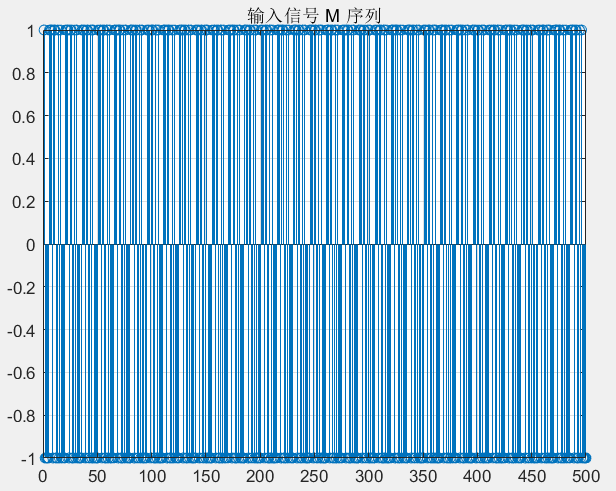
\includegraphics[width=.8\textwidth]{figure/输入信号M序列(迭代次数500).png} 
    \caption{输入信号M序列(迭代次数500)} % caption是图片的标题
    % \label{img} % 此处的label相当于一个图片的专属标志,目的是方便上下文的引用
\end{figure}

迭代过程中的参数估计误差如下图所示:
\begin{figure}[H]
    \centering % 居中 
    % 图片文件的相对路径
    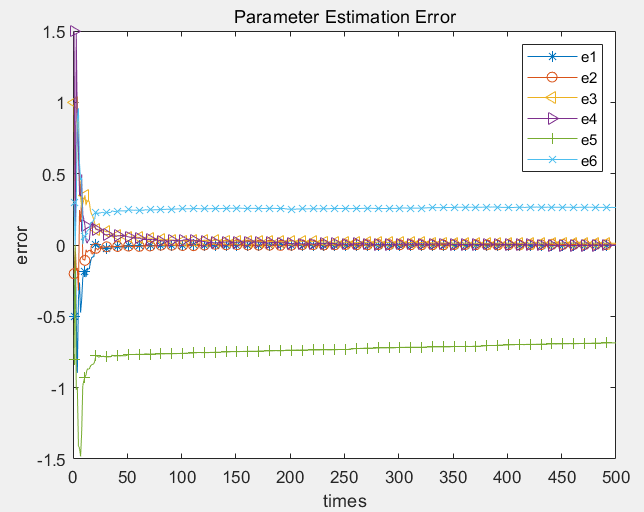
\includegraphics[width=.8\textwidth]{figure/递推极大似然-参数估计误差.png} 
    \caption{参数估计误差(迭代次数500)} % caption是图片的标题
    % \label{img} % 此处的label相当于一个图片的专属标志,目的是方便上下文的引用
\end{figure}

系统的输出误差如下图所示:
\begin{figure}[H]
    \centering % 居中 
    % 图片文件的相对路径
    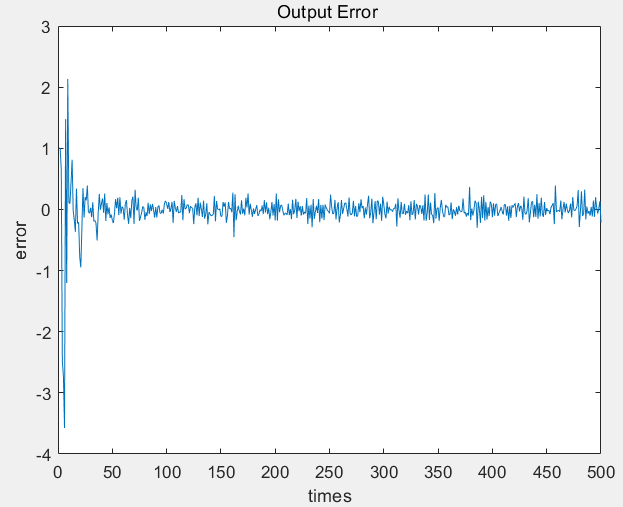
\includegraphics[width=.8\textwidth]{figure/递推极大似然-系统输出误差.png} 
    \caption{系统输出误差(迭代次数500)} % caption是图片的标题
    % \label{img} % 此处的label相当于一个图片的专属标志,目的是方便上下文的引用
\end{figure}

最终的参数估计如下:
\begin{table}[H] % 防止表格乱跑
\centering % 居中
\begin{tabular}{cccc} % 指明列数
    \toprule % 顶部粗线
    辨识参数 & 实际值 & 辨识值 & 误差百分比(\%) \\
    \midrule % 中间细线
    $a_1$ & -0.5 & -0.5015 & 0.3 \\
    $a_2$ & -0.2 & -0.2005 & 0.25 \\
    $b_1$ & 1.0 & 1.0048 & 0.48 \\
    $b_2$ & 1.5 & 1.4868 & 0.88 \\
    $d_1$ & -0.8 & -0.0517 & 93.54 \\ 
    $d_2$ & 0.3 & -0.0014 & 99.53 \\
    \bottomrule % 底部粗线
\end{tabular}
\caption{递推极大似然辨识结果(迭代次数500)} % 标题
\end{table}


%%%
\paragraph{迭代次数:2000次}~{}

采用M序列作为系统输入:
\begin{figure}[H]
    \centering % 居中 
    % 图片文件的相对路径
    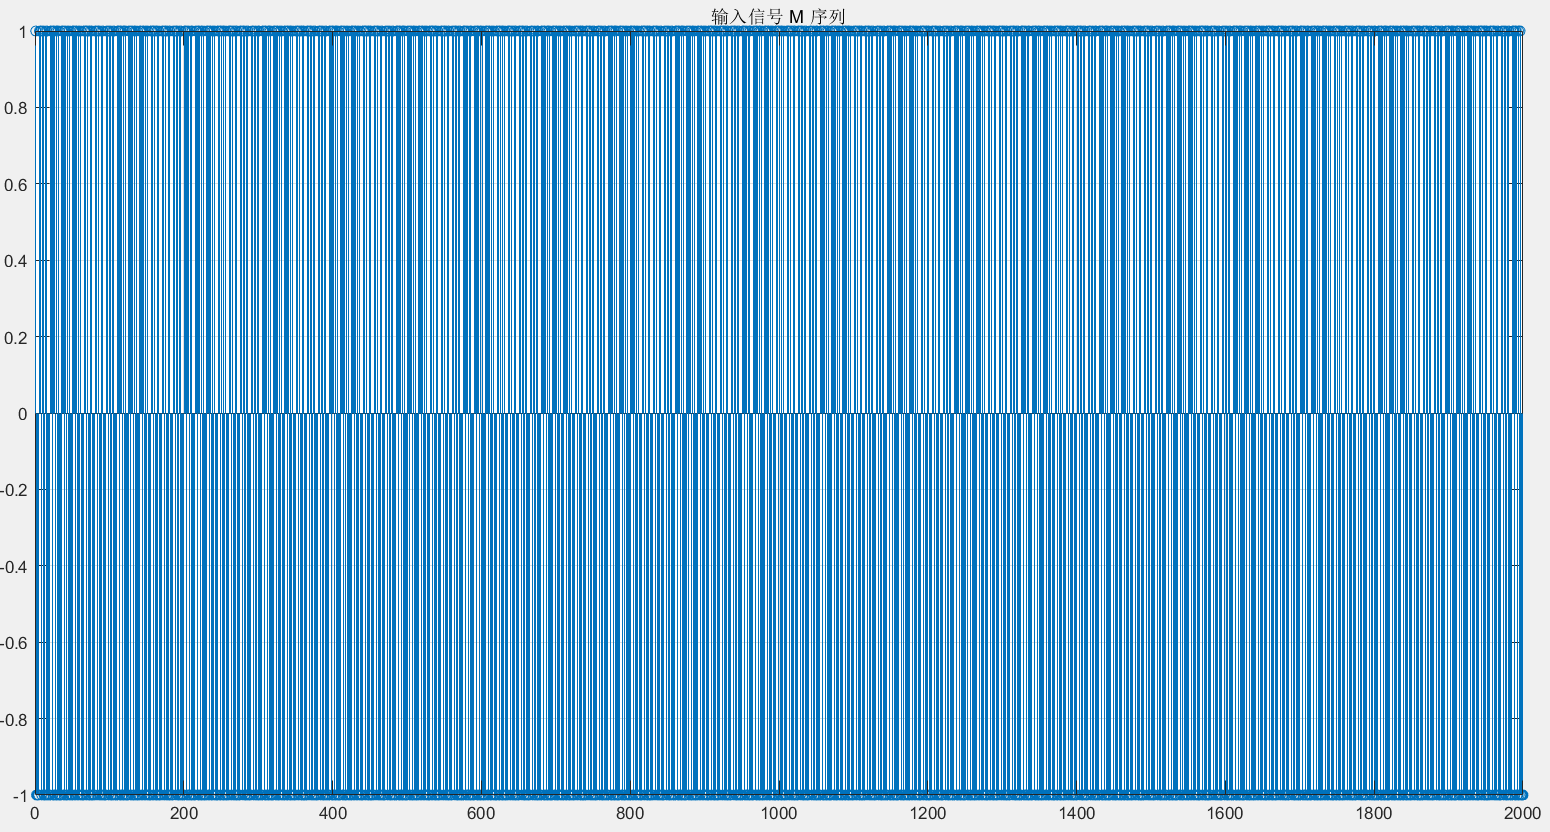
\includegraphics[width=.8\textwidth]{figure/输入信号M序列(迭代次数2000).png} 
    \caption{输入信号M序列(迭代次数2000)} % caption是图片的标题
    % \label{img} % 此处的label相当于一个图片的专属标志,目的是方便上下文的引用
\end{figure}

迭代过程中的参数估计误差:
\begin{figure}[H]
    \centering % 居中 
    % 图片文件的相对路径
    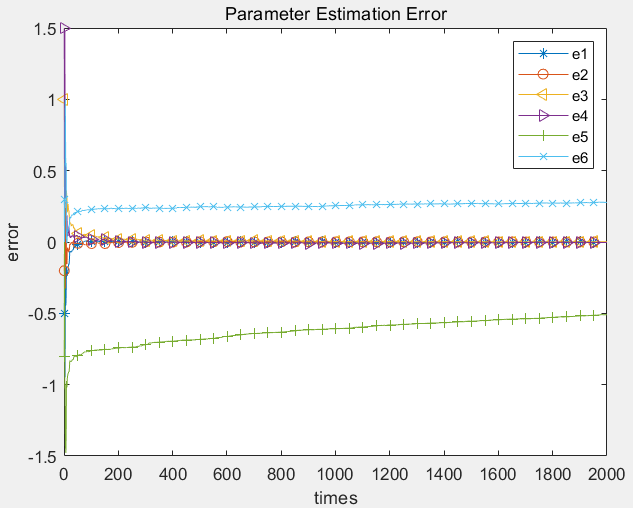
\includegraphics[width=.8\textwidth]{figure/递推极大似然-参数估计误差(迭代次数2000).png} 
    \caption{参数估计误差(迭代次数2000)} % caption是图片的标题
    % \label{img} % 此处的label相当于一个图片的专属标志,目的是方便上下文的引用
\end{figure}

系统的输出误差:
\begin{figure}[H]
    \centering % 居中 
    % 图片文件的相对路径
    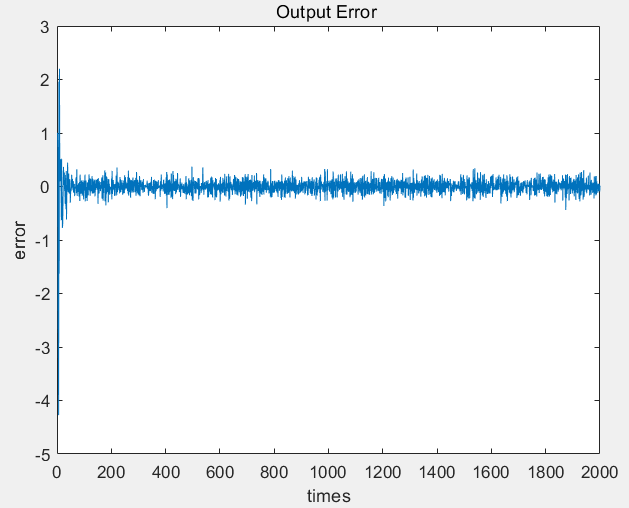
\includegraphics[width=.8\textwidth]{figure/递推极大似然-系统输出误差(迭代次数2000).png} 
    \caption{系统输出误差(迭代次数2000)} % caption是图片的标题
    % \label{img} % 此处的label相当于一个图片的专属标志,目的是方便上下文的引用
\end{figure}

最终的参数估计如下:
\begin{table}[H] % 防止表格乱跑
\centering % 居中
\begin{tabular}{cccc} % 指明列数
    \toprule % 顶部粗线
    辨识参数 & 实际值 & 辨识值 & 误差百分比(\%) \\
    \midrule % 中间细线
    $a_1$ & -0.5 & -0.4951 & 0.98 \\
    $a_2$ & -0.2 & -0.2052 & 2.6 \\
    $b_1$ & 1.0 & 0.9959 & 0.41 \\
    $b_2$ & 1.5 & 1.5076 & 0.51 \\
    $d_1$ & -0.8 & -0.2471 & 69.11 \\ 
    $d_2$ & 0.3 & 0.0043 & 98.57 \\
    \bottomrule % 底部粗线
\end{tabular}
\caption{递推极大似然辨识结果(迭代次数2000)} % 标题
\end{table}

%%%
\paragraph{结果分析}~{}
\begin{enumerate}
    \item 根据迭代过程中参数估计误差的变化情况可以看出,完成500次迭代以后参数$a_1,\ a_2,$ $ b_1,\ b_2$均已收敛至误差接近于零的状态,且随着迭代次数的继续增加,参数估计误差的收敛效果更加明显;
    \item 参数$d1,\ d2$的估计误差在经过2000迭代以后仍然保持在较高水平,这是因为由于噪声随机性(高斯白噪声),使得递推的极大似然参数估计对噪声项的参数估计效果很差。
\end{enumerate}


%%
\subsection{Newton-Raphson方法}
采用M序列作为系统输入,长度为12,如下图所示:
\begin{figure}[H]
    \centering % 居中 
    % 图片文件的相对路径
    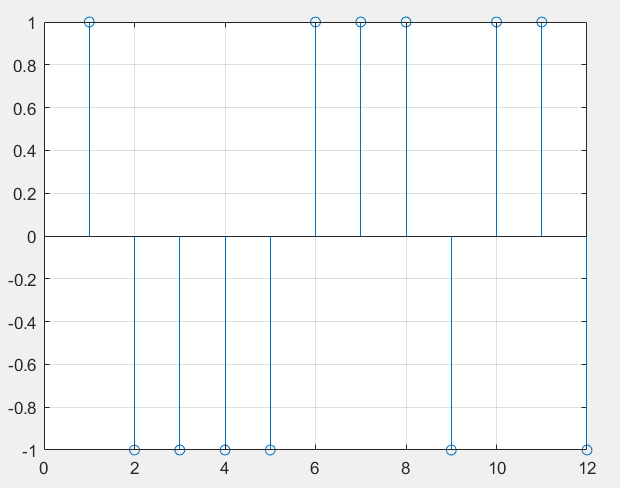
\includegraphics[width=.8\textwidth]{figure/newton_M序列输入.png} 
    \caption{Newton-Raphson方法 M序列输入} % caption是图片的标题
    % \label{img} % 此处的label相当于一个图片的专属标志,目的是方便上下文的引用
\end{figure}

迭代过程中的参数估计值如下图所示:
\begin{figure}[H]
    \centering % 居中 
    % 图片文件的相对路径
    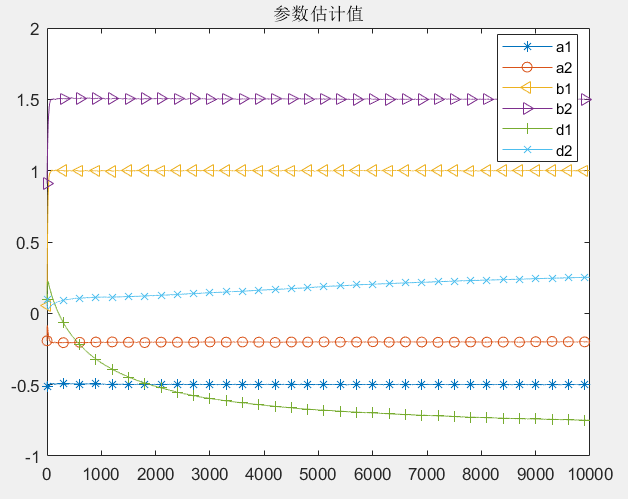
\includegraphics[width=.8\textwidth]{figure/newton_参数估计值.png} 
    \caption{Newton-Raphson方法 参数估计值} % caption是图片的标题
    % \label{img} % 此处的label相当于一个图片的专属标志,目的是方便上下文的引用
\end{figure}

参数估计误差如下图所示:
\begin{figure}[H]
    \centering % 居中 
    % 图片文件的相对路径
    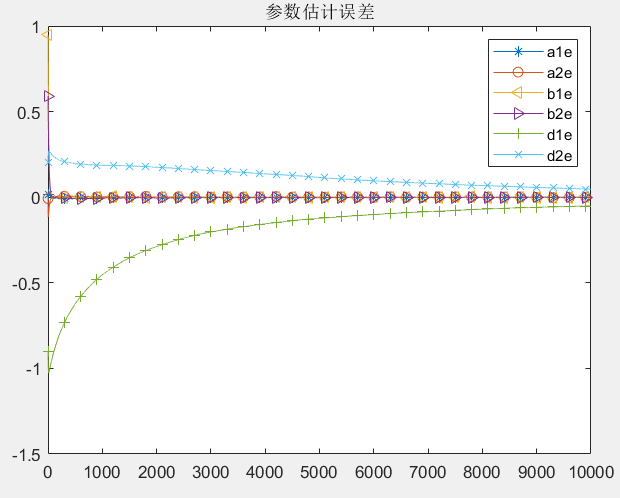
\includegraphics[width=.8\textwidth]{figure/newton_参数估计误差.png} 
    \caption{Newton-Raphson方法 参数估计误差} % caption是图片的标题
    % \label{img} % 此处的label相当于一个图片的专属标志,目的是方便上下文的引用
\end{figure}

最终的参数辨识结果如下:
\begin{table}[H] % 防止表格乱跑
\centering % 居中
\begin{tabular}{cccc} % 指明列数
    \toprule % 顶部粗线
    辨识参数 & 实际值 & 辨识值 & 误差百分比(\%) \\
    \midrule % 中间细线
    $a_1$ & -0.5 & -0.498588 & 0.2824 \\
    $a_2$ & -0.2 & -0.200589 & 0.2945 \\
    $b_1$ & 1.0 & 1.00164 & 0.164 \\
    $b_2$ & 1.5 & 1.49964 & 0.0240 \\
    $d_1$ & -0.8 & -0.750652 & 6.1685 \\ 
    $d_2$ & 0.3 & 0.252325 & 15.8917 \\
    \bottomrule % 底部粗线
\end{tabular}
\caption{Newton-Raphson方法辨识结果} % 标题
\end{table}


\paragraph{结果分析}~{}

相比递推的极大似然参数估计方法,Newton-Raphson方法对于噪声项的参数估计效果明显更好,收敛速度更快。由实验结果可以看到,经过10000次迭代以后,噪声项参数估计误差基本已收敛至零值。此外,根据本次实验结果可以看出,Newton-Raphson方法针对除噪声项参数之外的参数辨识效果较好,若对于噪声项参数的辨识精度有较高要求,则需要适当增大迭代次数。

%
\section{结论}
递推的极大似然参数估计方法对于除噪声项参数之外的其他参数的辨识效果较好,收敛速度快,而且精度高,可靠性好;但是对噪声项参数的辨识效果很差,这是由于噪声产生过程的随机性以及基于递推的极大似然参数估计的自身局限造成的。

相对来说,Newton-Raphson方法不仅在系统参数辨识上有着很高的精度,而且对于噪声项参数的辨识也有着较好的效果;其缺点在于,如果对噪声项参数的辨识精度有比较高的要求,则需要经过更多的迭代次数才能得到满意的结果,且完成一次迭代过程需要更多的数据作为支撑,运算量较大,对于数据获取的要求较高。

\end{document}